\documentclass[preprint]{elsarticle}

%%%
\usepackage{graphicx}
\usepackage{listings} 
\usepackage{amsmath}
\usepackage{listings} 
\usepackage{amsthm}
\usepackage{xspace}
\usepackage{latexsym,amssymb,stmaryrd}
\usepackage{color}
\usepackage{tikz}
\usepackage{prooftree}
\usepackage{proof}
\usetikzlibrary{calc}
\usetikzlibrary{shapes,snakes}
\usepackage{float}
%\floatstyle{boxed}
\restylefloat{figure}
\usepackage{wrapfig,subfig}
% !TEX root =main.tex

\theoremstyle{plain}

\newtheorem*{theorem*}{Theorem}
\newtheorem{theorem}{Theorem}
\newtheorem{lemma}[theorem]{{\bf Lemma}}
\newtheorem{definition}[theorem]{{\bf Definition}}
\newtheorem{proposition}[theorem]{{\bf Proposition}}
\newtheorem{example}[theorem]{{\bf Example}}
\renewenvironment{proof}[1][Proof]{\begin{trivlist}
\item[\hskip \labelsep {\bfseries #1}]}{\end{trivlist}}

%formatting code in the text
\newcommand*{\ttfamilywithbold}{\fontfamily{pcr}\selectfont}
\definecolor{darkRed}{RGB}{100,0,10}
\definecolor{darkBlue}{RGB}{10,0,100}
\lstset{language=Java,
  basicstyle=\ttfamily,%withbold,%\ttfamily,%\scriptsize,
  keywordstyle=\ttfamilywithbold\bfseries\color{darkRed},
  showstringspaces=false,
  mathescape=true,
  xleftmargin=0pt,
  xrightmargin=0pt,
  breaklines=false,
  breakatwhitespace=false,
  breakautoindent=false,
  linewidth=4\textwidth,% should be enough
%  identifierstyle=\idstyle
morekeywords={%
  mut,imm,
  read,capsule,lent
  }%
 }

%marco
\newcommand{\Q}{\lstinline}

%tipografiche
\newcommand{\refToFigure}[1]{Figure~\ref{fig:#1}}
\newcommand{\refToSection}[1]{Section~\ref{sect:#1}}
\newcommand{\refToLemma}[1]{Lemma~\ref{lemma:#1}}
\newcommand{\refToTheorem}[1]{Theorem~\ref{theo:#1}}
\newenvironment{ProofOf}[2]{\noindent{\it Proof of \refToTheorem{#1} (#2)}.}{}
\newcommand{\Space}{\hskip 0.8em}
\newcommand{\HSep}{\hbox to \textwidth{\bf\hrulefill}}
\newcommand{\qued}{\ensuremath{\hfill \square}}

%matematiche generali
\newcommand{\Tuple}[1]    {\langle{#1}\rangle}
\newcommand{\Pair}[2]     {\Tuple{{#1},{#2}}}
\newcommand{\Triple}[3]     {\Tuple{{#1},{#2},{#3}}}
\newcommand{\FourTuple}[4]     {\Tuple{{#1},{#2},{#3},{#4}}}
\newcommand{\SubstFun}[2]{#1[#2]}

%metaregole
\newcommand{\Rule}[3]{\displaystyle                  
\frac{#1}{#2}        %  #1 = premesse (modo math) %  #2 = conseguenza (modo math)
{#3}     %  #3 = side conditions (modo math)
}

\newcommand{\NamedRule}[4]{\scriptstyle{\textsc{(#1)}}
\displaystyle                  %  #1 = nome regola
\frac{%
\begin{array}{l}#2\end{array}%
}{#3}        %  #2 = premesse (modo math) %  #3 = conseguenza (modo math)
\begin{array}{l}#4\end{array}     %  #4 = side conditions (modo math)
}
\newcommand{\SmallNamedRule}[4]{\scriptstyle{\textsc{(#1)}}
\displaystyle                  %  #1 = nome regola
\frac{%
\begin{array}{l}#2\end{array}%
}{#3}\Space           %  #2 = premesse (modo math) %  #3 = conseguenza (modo math)
\scriptstyle{\begin{array}{l}#3\end{array}}     %  #4 = side conditions (modo math)
}

%metaregole in un asola riga
\newcommand{\NamedRuleOL}[3]{\scriptstyle{\textsc{(#1)}}
\displaystyle                  %  #1 = nome regola
{%
\begin{array}{l}#2\end{array}}\           
\begin{array}{l}#3\end{array}     %  #3 = side conditions (modo math)
}
\newcommand{\SmallNamedRuleOL}[3]{\scriptstyle{\textsc{(#1)}}
\displaystyle                  %  #1 = nome regola
{#2}       % 
\scriptstyle{\begin{array}{l}#3\end{array}}     %  #3 = side conditions (modo math)
}

\newcommand{\rn}[1]{{\scriptsize (\textsc{#1})}}					% Rule name

%grammatiche
\newenvironment{grammatica}{$\begin{array}{lcll}}{\end{array}$}
\newcommand{\produzione}[3]{#1&::=&#2&\mbox{#3}}
\newcommand{\produzioneinline}[2]{#1::=#2}
\newcommand{\seguitoproduzione}[2]{&&#1&\mbox{#2}}
\newcommand{\terminale}[1]{\texttt{#1}}
\newcommand{\metavariable}[1]{\mathit{#1}}

%metavariabili
\newcommand{\n}{\metavariable{n}}
\newcommand{\cd}{\metavariable{cd}}
\newcommand{\cds}{\metavariable{cds}}
\newcommand{\fd}{\metavariable{fd}}
\newcommand{\fds}{\metavariable{fds}}
\newcommand{\md}{\metavariable{md}}
\newcommand{\mds}{\metavariable{mds}}
\newcommand{\x}{\metavariable{x}}
\newcommand{\y}{\metavariable{y}}
\newcommand{\z}{\metavariable{z}}
\newcommand{\xs}{\metavariable{xs}}
\newcommand{\ys}{\metavariable{ys}}
\newcommand{\zs}{\metavariable{zs}}
\newcommand{\m}{\metavariable{m}}
\newcommand{\e}{\metavariable{e}}
\newcommand{\es}{\metavariable{es}}
\newcommand{\C}{\metavariable{C}}
\newcommand{\D}{\metavariable{D}}
\newcommand{\f}{\metavariable{f}}
\newcommand{\dec}{\metavariable{d}}
\newcommand{\decs}{\metavariable{ds}}
\newcommand{\X}{\metavariable{X}} %insieme di variabili

%%terminali
\newcommand{\this}{\terminale{this}}
\newcommand{\mutable}{\terminale{mut}}
\newcommand{\imm}{\terminale{imm}}
\newcommand{\lent}{\terminale{lent}}
\newcommand{\readable}{\terminale{read}}
\newcommand{\capsule}{\terminale{capsule}}

%%costrutti sintattici
\newcommand{\Field}[2]{#1\ #2\terminale{;}}
\newcommand{\MethDec}[5]{{#1\ #2\ \terminale{(}#3,#4\terminale{)}\ \terminale{\{}#5\terminale{\}}}}
\newcommand{\Param}[2]{#1\ #2}
\newcommand{\FieldAccess}[2]{#1\terminale{.}#2}
\newcommand{\MethCall}[3]{#1\terminale{.}#2\terminale{(}#3\terminale{)}}
\newcommand{\FieldAssign}[3]{#1\terminale{.}#2\terminale{=}#3}
\newcommand{\ConstrCall}[2]{\terminale{new}\,#1\!\terminale{(}#2\terminale{)}}
\newcommand{\Block}[2]{\terminale{\{}#1\ #2\terminale{\}}}
\newcommand{\Dec}[3]{#1\,#2\terminale{=}#3\terminale{;}}
%\newcommand{\Field}[2]{#1\ #2}
%\newcommand{\PrExp}[2]{(#1)\,#2}
\newcommand{\Sequence}[2]{#1\terminale{;} #2}
\newcommand{\emptyDvs}{\epsilon}

%%type system
\newcommand{\WellFormedTypeCtx}[1]{\vdash#1}
\newcommand{\Encoded}[2]{#1\rightsquigarrow #2}
\newcommand{\MutGroup}{\metavariable{xs}}
\newcommand{\intType}{\terminale{int}}
\newcommand{\T}{\metavariable{T}}
\newcommand{\TPrime}{{\T}'}
\newcommand{\Type}[2]{#1\,#2}
\newcommand{\IsWellTyped}[1]{\vdash #1}
\newcommand{\TypeCheckGround}[2]{\vdash #1:#2}
\newcommand{\TypeCheck}[5]{#1;#2;#3\vdash #4:#5}
\newcommand{\AuxTypeCheck}[6]{#1;#2\,[#3];#4\vdash #5:#6}
\newcommand{\TypeCheckShort}[3]{#1\vdash #2:#3}
\newcommand{\TypeDec}[2]{#2{:}#1}
\newcommand{\LentLocked}{\metavariable{xss}}
\newcommand{\StronglyLocked}{\metavariable{ys}}
\newcommand{\Reduct}[2]{#1_{|#2}}
\newcommand{\Extends}[3]{#1\sqsubseteq_{#2}#3}
\newcommand{\LentVars}[1]{\aux{lentVars}(#1)}
\newcommand{\MutVars}[1]{\aux{mutVars}(#1)}
\newcommand{\LessEq}[2]{#1\sqsubseteq#2}

%%valori e contesti
\newcommand{\dv}{\metavariable{dv}}
\newcommand{\dvs}{\metavariable{dvs}}
\newcommand{\Ctx}[1]{\ctx[#1]}
\newcommand{\XCtx}[1]{\Xctx[#1]}
\newcommand{\CtxP}[1]{\ctxP[#1]}
\newcommand{\CtxS}[1]{\ctxS[#1]}
\newcommand{\XCtxP}[1]{\XctxP[#1]}
\newcommand{\ctx}{{\cal{E}}}
\newcommand{\genCtx}{{\cal{G}}}
\newcommand{\GenCtx}[1]{\genCtx[#1]}
\newcommand{\genCtxP}{{\cal{G'}}}
\newcommand{\GenCtxP}[1]{\genCtxP[#1]}
\newcommand{\Xctx}{{\cal{C}}}
\newcommand{\ctxP}{{\cal{E}'}}
\newcommand{\ctxS}{{\cal{E}''}}
\newcommand{\XctxP}{{\cal{C}'}}
\newcommand{\emptyctx}{[\ ]}
\newcommand{\val}{\metavariable{v}}
\newcommand{\stVal}{\metavariable{rv}}
\newcommand{\valPrime}{\metavariable{u}}
\newcommand{\vals}{\metavariable{vs}}
\newcommand{\vs}{\metavariable{vs}}

%%riduzione
\newcommand{\reduce}[2]{#1\longrightarrow#2}
%\newcommand{\reducestar}[2]{#1\longrightarrow^\star#2}
\newcommand{\Subst}[3]{#1[#2/#3]}
\newcommand{\Update}[4]{{#1[#2.#3{=}#4]}}

%%equivalenza
\newcommand{\congruence}[2]{{#1}\cong{#2}}

%%funzioni ausiliarie
\newcommand{\extractMod}[1]{\mu^{#1}}
\newcommand{\aux}[1]{\textsf{#1}}
\newcommand{\notRef}[1]{{\aux{notVar}}(#1)}
\newcommand{\extractDec}[2]{\aux{dec}(#1,#2)}
\newcommand{\extractType}[2]{\aux{type}(#1,#2)}
\newcommand{\typeOf}[1]{\aux{type}(#1)}
\newcommand{\extractField}[3]{\aux{get}(#1,#2,#3)}
\newcommand{\fieldOf}[2]{\aux{get}(#1,#2)}
\newcommand{\fields}[1]{\aux{fields}(#1)}
\newcommand{\method}[2]{{\aux{method}(#1,#2)}}
\newcommand{\FV}[1]{\aux{FV}(#1)}
\newcommand{\HB}[1]{\aux{HB}(#1)}
\newcommand{\dom}[1]{\aux{dom}(#1)}
\newcommand{\domMut}[1]{\aux{dom}^\mutable(#1)}
\newcommand{\domLent}[1]{\aux{dom}^\lent(#1)}
\newcommand{\domGeqMut}{{\aux{dom}^{\geq\terminale{mut}}}}
\newcommand{\ImmClosed}[2]{#1\models\aux{imm-closed}(#2)}
\newcommand{\allImm}[1]{\forall^\imm(#1)}
\newcommand{\allMut}[1]{\forall^{\geq\mutable}(#1)}
\newcommand{\noCapture}[2]{#1{\parallel}#2}

%----------scaled enviroment-------------
\newsavebox{\saveScaled}
\newcommand*{\varScalableEnvironmentWidth}{1}
\newcommand*{\varScalableEnvironmentHeight}{1}
\newenvironment{Scaled}[2]{%
  \renewcommand*{\varScalableEnvironmentWidth}{#1}
  \renewcommand*{\varScalableEnvironmentHeight}{#2}
  \begin{lrbox}{\saveScaled}
  }{
  \end{lrbox}
  \noindent\scalebox{\varScalableEnvironmentWidth}[\varScalableEnvironmentHeight]{\usebox{\saveScaled}}
  }
%
%
%%%% MACRO PAOLA
%
\newcommand{\storableVal}{right-value}
\newcommand{\storableValues}{right-values}
\newcommand{\storableVals}{right-values}
\newcommand{\preRedex}{{\rho}}
\newcommand{\deriv}{{\cal D}}
\newcommand{\WFrv}[1]{\models#1}
\newcommand{\WFdvs}[1]{\models#1}
\newcommand{\WFdv}[1]{\models_{st}#1}
\newcommand{\WFval}[1]{\PG{\models_{st}#1}}
%\newcommand{\WFdvMod}[2]{\models_{#1}#2}
\newcommand{\dependVar}[2]{\aux{dpd}(#1,#2)}
\newcommand{\mutDvs}[1]{\aux{mutDvs}(#1)}
%\newcommand{\TypeEnv}[1]{\aux{tenv}(#1)}
\newcommand{\TypeEnv}[1]{\Gamma_{\!#1}}
\newcommand{\TypeEnvDec}[1]{\aux{tenv}(#1)}
\newcommand{\DecsOK}[4]{#1;#2;#3\vdash #4\,{\tt OK}}
\newcommand{\AuxDecsOK}[5]{#1;#2[#3];#4\vdash #5\,{\tt OK}}
\newcommand{\leqLL}{\sqsubseteq}
\newcommand{\Depends}[2]{\aux{dpd}(#1,#2)}

\newcommand{\capsulectx}{\decctx{\cx}}
\newcommand{\immctx}{\decctx{\ix}}
\newcommand{\Capsulectx}[1]{\Decctx{\cx}{#1}}
\newcommand{\Immctx}[1]{\Decctx{\ix}{#1}}
\newcommand{\CapsulectxP}[1]{{\cal C}'_{\cx}[#1]}
\newcommand{\ImmctxP}[1]{{\cal C}'_{\ix}[#1]}
\newcommand{\ImmctxS}[1]{{\cal C}''_{\ix}[#1]}
\newcommand{\decctx}[1]{{\cal C}\!_{#1}}
\newcommand{\Decctx}[2]{{\cal C}\!_{#1}[#2]}
\newcommand{\DecEvCtx}[2]{#1_{#2}}

\newcommand{\mux}{\mu\hspace{.015cm}\x}
\newcommand{\cx}{{\tt c}\hspace{.015cm}\x}
\newcommand{\ix}{{\tt i}\hspace{.015cm}\x}

%\newcommand{\Extend}[2]{{\it Xtd}(#1,#2)}
\newcommand{\Range}[3]{\forall#1\in#2..#3}

%\newcommand{\subderivation}[2]{#1{\Longrightarrow}#2}

%\newenvironment{myitemize}
%               {\begin{itemize}\vspace{-2pt}\topsep0pt\parskip0pt\partopsep0pt\itemsep0pt\leftmargin-100pt\itemsep-1pt\labelwidth0pt\labelsep3pt}
%               {\vspace{-1pt}\end{itemize}}
               
%\newtheorem*{theorem*}{Theorem}

\newcommand{\cOrx}{w}

\newcommand{\connected}[3]{#2\stackrel{#1}{\longrightarrow}#3}
%\newcommand{\TypeOf}[3]{{#1}_{#2}(#3)}





\begin{document}\newif\ifsubmit
%\submittrue
\submitfalse
\ifsubmit
\newcommand{\EZ}[1]{#1}
\newcommand{\EZComm}[1]{}
\newcommand{\PG}[1]{#1}
\newcommand{\PGComm}[1]{}
\newcommand{\MS}[1]{#1}
\newcommand{\MSComm}[1]{}
\newcommand{\JC}[1]{#1}

\newcommand{\JCComm}[1]{}
\else
\newcommand{\EZ}[1]{\textcolor{blue}{#1}}

\newcommand{\EZComm}[1]{{\scriptsize \textcolor{blue}{[Elena{:} #1]}}}

%\newcommand{\PG}[1]{\textcolor{magenta}{#1}}
\newcommand{\PG}[1]{\textcolor{blue}{#1}}

\newcommand{\PGComm}[1]{{\scriptsize \textcolor{magenta}{[Paola{:} #1]}}}
\newcommand{\MS}[1]{\textcolor{green}{#1}}
\newcommand{\MSComm}[1]{{\scriptsize \textcolor{green}
{[MS{:} #1]}}}
\newcommand{\JC}[1]{\textcolor{red}{#1}}
\newcommand{\JCComm}[1]{{\scriptsize \textcolor{red}
{[JC{:} #1]}}}

\fi


\begin{frontmatter}

\title{{Flexible recovery of uniqueness and immutability\\
(Extended Version)}}


\author[pg]{Paola Giannini\corref{cor1}}
\ead{giannini@di.unipmn.it}

\author[ms]{Marco Servetto}
\ead{marco.servetto@ecs.vuw.ac.nz}

\author[ez]{Elena Zucca}
\ead{elena.zucca@unige.it}

\author[ms]{James Cone}
\ead{james.cone@ecs.vuw.ac.nz}


\cortext[cor1]{Principal corresponding author}


\address[ms]{School of Engineering and Computer Science, Victoria University of Wellington, Gate 6, Kelburn Parade
Wellington, New Zealand}
\address[pg]{Computer Science Institute, DiSIT, Universit\`a del Piemonte Orientale, viale Teresa Michel 11,  Alessandria, Italy\footnote{This original research has the financial support of the Universit\`a  del Piemonte Orientale.}
}
\address[ez]{DIBRIS, Universit\`a di Genova, Via Dodecaneso 35, Genova, Italy}
 
\begin{abstract}
We present an imperative object calculus where types are annotated with qualifiers for aliasing {and mutation} control.  There are two key novelties with respect to similar proposals. {First, the type system is very expressive. Notably, it adopts the \emph{recovery} approach, that is, using the
type context to justify strengthening types, greatly improving its power by permitting to recover uniqueness and immutability properties even in presence of other references. This is achieved by rules which restrict the use of such other references in the portion of code which is recovered.  Second, execution is modeled by a non standard operational model, where} 
properties of qualifiers can be directly expressed on source terms, rather than as invariants on an auxiliary structure which mimics physical memory. Formally, this is achieved by the block construct, introducing local variable declarations, which, when evaluated, play the role of store.
\end{abstract}


\begin{keyword}
{Type systems; Imperative calculi; Immutability; Aliasing}
\end{keyword}
\end{frontmatter}


\section{Introduction}
\label{sec:intro}

\subsection{Motivation}

Reliable estimation of a signal (or image) from nonlinear observations is of fundamental interest to several signal processing and machine learning applications. However, such an estimation is confounded by cases where the nonlinearity in each observation is well-modeled by a \emph{periodic} function such as a sinusoidal function, or sawtooth function, or a square-wave function. Periodic functions are many-to-one mappings, and inverting them can be challenging.

Our focus in this paper is a special kind of periodic nonlinear observation model encountered in high-dynamic range (HDR) imaging. It is well known that real world scenes contain a large range of brightness levels. However, due to hardware limitations, not all brightness levels can be accurately captured using conventional photography; if tuned incorrectly, most scene intensity levels can lie in the saturation region of the image sensors, causing loss of scene information. Similar problems arise in the case of multiplexed imaging systems, such as lensless and coded aperture imaging~\cite{codedaperture,asif2017flatcam}.

%While increasing the dynamic range can solve this problem, it is an impractical strategy since imaging sensors need to have infinite dynamic range, which is infeasible. 
One solution is to increase the dynamic range of the image sensors, but this can lead to expensive hardware. An alternative solution is to deploy a special type of image sensor that {wraps} the observed intensity value at a pixel over a given dynamic range. This is analogous to the familiar \emph{modulo} operation with respect to a parameter $R$, and we call this stylized imaging system a \emph{modulo camera}~\cite{ICCP15_Zhao}.  
Fig.~\ref{fig:func}(a) (black) depicts the modulo nonlinearity, and a major challenge is to undo the effect of this transformation for each observed pixel.

An added challenge in HDR imaging arises due to \emph{quantization}. In fact, the ``true" observations in a modulo camera are quantized versions of the (idealized) modulo observation, and the errors caused in the quantization propagates into the estimation process. Loss of information in the quantization process is unavoidable in principle, and the effect of quantization is magnified with fewer quantization levels. In acquisition systems with low bit-depth, such estimation errors can be very pronounced. Fig.~\ref{fig:func}(a) (cyan) depicts the quantization nonlinearity incurred during the observation process.

\subsection{Setup}

We formalize the above discussion as follows. Assume $\mathcal{X} \subseteq \R^{n}$ to be a given (known) subset in the data space, and consider a signal (or image) $x \in \mathcal{X}$. We model (possible) multiplexing operations and gain adjustments as linear transformations, denoted by $A\in\mathbb{R}^{p\times n}$ and $C\in\R^{m\times p}$ respectively. The composite observation model becomes:
\begin{equation}
\label{quan_obs}
u=f(Ax),~y=Q(Cu),
\end{equation}
where $f(\cdot)=\mod(\cdot,R)$ denotes the modulo function with respect to a range parameter $R$ and $Q(\cdot)$ denotes a quantization function. In this paper, we consider a 1-bit quantization function with only two levels, $0$ and $1$. A representative example is shown in Fig.\ \ref{fig:func} where $A$ and $C$ are identity operators. In  Figs~\ref{fig:func}(c)  and~\ref{fig:func}(d), the outputs of the functions $f$ and $Q$ are displayed when a test grayscale image (Fig.\ \ref{fig:func}(a)) is used in the input. Our overall objective is to estimate the original signal $x$ from the set of measurements $y$. 

%%%%%%%%%%%%%%%%%%%%%%%%%%%%%%%%%%%%%
\begin{figure}[t]
	
	\begin{center}
		\begingroup
		\setlength{\tabcolsep}{0.1pt} % Default value: 6pt
		\renewcommand{\arraystretch}{.1} % Default value: 1
		\begin{tabular}{ccc}      %{c@{\hskip .1pt}c@{\hskip .1pt}c}
			\multicolumn{3}{c}{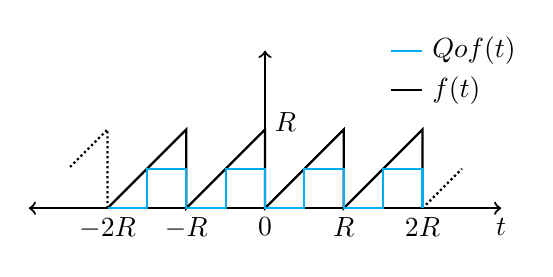
\begin{tikzpicture}
				\draw[<->,thick] (-3,0)--(3,0) node[anchor=north]{$t$};
				\draw (0,0) node[anchor=north]{$0$};
				\draw (0,1.1) node[anchor=west] {$R$};
				\draw (1,0) node[anchor=north]{$R$};
				\draw (2,0) node[anchor=north] {$2R$};
					\draw (-1,0) node[anchor=north]{$-R$};
				\draw (-2,0) node[anchor=north] {$-2R$};
				\draw[] (2,2) node[anchor=west] {{$Qof(t)$}};
				\draw[cyan,thick] (1.6,2) -- (2,2);
				%\draw [densely dotted,thick] (-2.5,1)--(3,1);
				\draw[->,thick] (0,0)--(0,2);
				\draw[] (2,1.5) node[anchor=west] {{$f(t)$}};
				\draw[thick] (1.6,1.5) -- (2,1.5);
				\draw[thick] (-2,0) --(-1,1)-| (-1,0) -- (0,1) -| (0,0) --(1,1)-| (1,0) -- (2,1) -| (2,0);
				\draw[densely dotted,thick] (2,0)--(2.5,0.5);
				\draw[densely dotted,thick] (-2,0)|-(-2,1) -- (-2.5,0.5);
				\draw[thick, cyan] (-2,0) -- ++(0.5,0)-| ++(0,0.5) -- ++(0.5,0) -| ++(0,-0.5) -- ++(0.5,0)-| ++(0,0.5) -- ++(0.5,0) -| ++(0,-0.5) -- ++(0.5,0)-| ++(0,0.5) -- ++(0.5,0) -| ++(0,-0.5) -- ++(0.5,0)-| ++(0,0.5) -- ++(0.5,0) -| ++(0,-0.5);
				\end{tikzpicture}}\\
			\multicolumn{3}{c}{(a)}\\
			\includegraphics[trim = 10mm 60mm 25mm 40mm,clip, width = 0.32\linewidth]{./orgimg.pdf}&
			\includegraphics[trim = 10mm 60mm 25mm 40mm,clip, width = 0.32\linewidth]{./modimg.pdf}&
			\includegraphics[trim = 10mm 60mm 25mm 40mm,clip,width = 0.32\linewidth]{./quantimg.pdf} \\
			(b) & (c) & (d)
		\end{tabular}
		\endgroup
	\end{center}
	\caption{\small{\emph{ (a) Modulo function, $f(t) = \mod(t,R)$ and quantized modulo function, $Qof(t)$; (b,c,d) Depiction of forward model. An input image (b) is transformed via a modulo function $f(t) = \mod(t,R)$, to (c). Such a ``modulo" image is further quantized to obtain (d).}}}
	\label{fig:func}
\end{figure}
%%%%%%%%%%%%%%%%%%%%%%%%%%%%%%%%%%%%%%%%%%%%%%%%%%

\subsection{Our contributions}

Clearly, the above estimation procedure is challenging due to the highly non-invertible nature of the observation model. In this paper, we design a systematic approach that takes some initial steps towards resolving this challenge. Our overarching assumption is that the measurement operations $A$ and $C$ are part of the design space. The core idea in our approach is that a very small, but carefully designed, non-adaptive set of measurements can support efficient estimation of the unknown signal.

Our approach follows stagewise. First, we consider the problem of inverting the quantization function, i.e., recovering $u$ from $y = Q(Cu)$. We demonstrate the existence of a linear operator $C$ (together with an efficient reconstruction algorithm) that supports such an inversion. Specifically, our operator $C$ obeys a particular block-diagonal form with weights chosen according to a harmonic progression; see Section~\ref{sec:Model} for details. We only consider 1-bit quantization functions, but similar ideas can presumably be extended for a higher number of quantization levels. In addition, our method supports the criterion of \emph{consistent reconstruction} as defined in \cite{jacques2011dequantizing}.

Next, we consider the problem of inverting the modulo operation, i.e., recovering $x$ from $u = f(Ax)$.  We propose an algorithm that builds upon the approach proposed in \cite{SoltaniHegde_ICASSP16}. In particular, we show that if the operator $A$ satisfies a certain \emph{factorization} $A = DB$, then $f$ can be stably inverted. To enable efficient inversion, the matrix $D$ must also be block-diagonal with weights chosen either randomly, or according to a geometric progression. In the former case, the reconstruction algorithm is an extension of the approach of~\cite{SoltaniHegde_ICASSP16}, while in the latter case the reconstruction follows the approach of~\cite{ICCP15_Zhao}.

The above two-stage procedure can be easily adapted to the case where we have some prior knowledge of the original signal $x$. This enables our approach to be used in conjunction with compressive imaging architectures. Common priors used in compressive imaging include \emph{sparsity} in some known orthonormal basis~\cite{foucart2013}. Note that our measurements are highly quantized and the total ``bit" complexity of our observations is far smaller than conventional techniques. Therefore, within our framework, one can choose to increase the number of quantizer measurements (rows of $C$) and/or modulo measurements (rows of $D$) in order to achieve better estimation performance.


Fig.~\ref{fig:demo} displays some representative results using our approach. We begin with a standard ``Peppers" image, compute a modulo transformation with three multiplexed measurements per pixel, and further modulate it with a sequence of three harmonic multipliers per measurement before passing it through a 1-bit quantizer. (In words, the overall ``oversampling factor" in our method is $9\times$.) The final binary measurements displayed in Fig.\ \ref{fig:demo}(a) are given as inputs to our reconstruction algorithm. The results from the first and second stages are displayed as images in Fig.\ \ref{fig:demo}(b). As is visually evident, our method is able to successfully reconstruct the image, as displayed in Fig.\ \ref{fig:demo}(c). 


\begin{figure}[t]
	\begin{center}
		\begingroup
		\setlength{\tabcolsep}{1pt} % Default value: 6pt
		\renewcommand{\arraystretch}{.1} % Default value: 1
		{\setlength{\tabcolsep}{1mm}
		\begin{tabular}{ccc|c|c}      %{c@{\hskip .1pt}c@{\hskip .1pt}c}
			\centering
			\includegraphics[trim = 30mm 60mm 40mm 65mm,clip, width = 0.15\linewidth]{./quant11.pdf}&
			\includegraphics[trim = 30mm 60mm 40mm 65mm,clip, width = 0.15\linewidth]{./quant12.pdf}&
			\includegraphics[trim = 30mm 60mm 40mm 65mm,clip, width = 0.15\linewidth]{./quant13.pdf}&
			\includegraphics[trim = 90mm 125mm 90mm 120mm,clip, width = 0.18\linewidth]{./mod11.pdf}&
				\multirow{3}{20mm}{\includegraphics[trim = 90mm 85mm 90mm 120mm,clip, width = \linewidth]{./dms_img.pdf}}\\
			\includegraphics[trim = 30mm 60mm 40mm 65mm,clip, width = 0.15\linewidth]{./quant21.pdf}& 
			\includegraphics[trim = 30mm 60mm 40mm 65mm,clip, width = 0.15\linewidth]{./quant22.pdf}&
			\includegraphics[trim = 30mm 60mm 40mm 65mm,clip, width = 0.15\linewidth]{./quant23.pdf}&
			\includegraphics[trim = 90mm 125mm 90mm 120mm,clip, width = 0.18\linewidth]{./mod21.pdf}&\\
			\includegraphics[trim = 30mm 50mm 40mm 65mm,clip, width = 0.15\linewidth]{./quant31.pdf}& 
			\includegraphics[trim = 30mm 50mm 40mm 65mm,clip, width = 0.15\linewidth]{./quant32.pdf}&
			\includegraphics[trim = 30mm 50mm 40mm 65mm,clip, width = 0.15\linewidth]{./quant33.pdf}& 
			\includegraphics[trim = 90mm 125mm 90mm 120mm,clip, width = 0.18\linewidth]{./mod31.pdf}&\\[1pt]
			\multicolumn{3}{c|}{(a)} &(b)&{\centering(c)}
		\end{tabular}}
		\endgroup
	\end{center}
	\caption{\small{\emph{Illustration of our approach. A given input image is modulated pixel-wise with three pre-chosen weights, passed through a modulo sensor, modulated again pixel-wise with three weights, and quantized to binary images. The resulting observations are shown in (a). The images in (b) and (c) represent the reconstruction of the modulo images, $\widehat{u}$ and the final image, $\widehat{x}$, respectively.}}}
	
	\label{fig:demo}
\end{figure}



\section{Informal presentation of the {calculus}}\label{sect:informal}
Syntax and types are given in \refToFigure{syntax}.  We assume sets of \emph{variables} $\x$, $\y$, $\z$, \emph{class names} $\C$, \emph{field names} $\f$, and \emph{method names} $\m$. 
We adopt the convention that a metavariable which ends by $\metavariable{s}$ is implicitly defined as a (possibly empty) sequence, {for example} {$\decs$ is defined by $\produzioneinline{\decs}{\epsilon\mid \dec\ \decs}$}, where $\epsilon$ denotes the empty sequence.

\begin{figure}
\framebox{{\small \begin{grammatica}
\produzione{\cd}{\terminale{class}\ \C\ \terminale{\{}\fds\ \mds \terminale{\}}}{class declaration}\\*
\produzione{\fd}{
\Field{\Type{\imm}{\C}}{\f}
\mid
\Field{\Type{\mutable}{\C}}{\f}\mid\Field{\intType}{\f}}{field declaration}\\*
\produzione{\md}{\MethDec{\T}{\m}{{\mu}}{\T_1\,\x_1,\ldots,\T_n\,\x_n}{\e}}{method declaration}\\*
\produzione{\e}{\x\mid\FieldAccess{\e}{\f}\mid\MethCall{\e}{\m}{\es}\mid\FieldAssign{\e}{\f}{\e}\mid\ConstrCall{\C}{\es}\mid\Block{\decs}{\e}}{expression}\\*
\produzione{\dec}{\Dec{\T}{\x}{\e}}{variable declaration}\\*
\\
\produzione{\T}{\Type{\mu}{\C}\mid\intType}{type}\\*
\produzione{\mu}{\mutable\mid\imm\mid\capsule\mid\lent\mid\readable}{{(type)} qualifier}\\*
\\
\produzione{\dv}{\Dec{\T}{\x}{\stVal}}{evaluated declaration}\\
%\produzione{{\valPrime,}\val}{{\x\mid\ConstrCall{\C}{\vals}\mid\Block{\dvs}{\val}}}{value}\\*
\produzione{\stVal}{\ConstrCall{\C}{\xs}\mid\Block{\dvs}{\x}\mid\Block{\dvs}{\ConstrCall{\C}{\xs}}}{\storableVal}
\end{grammatica}
}}
\caption{Syntax and types}\label{fig:syntax}
\end{figure}

The syntax mostly follows Java and Featherweight Java (FJ) \cite{IgarashiEtAl01}. A class declaration consists of a class name, a sequence of field declarations and a sequence of method declarations. A field declaration consists of a field type and a field name.
 A method declaration consists, as in FJ, of a return type, a method name, a list of parameter names with their types, and a body which is an expression. {However, there is an additional component: the type qualifier for $\this$, which is {written as additional (first) element of the parameter list}.}
  As in FJ, we assume for each class a canonical constructor whose parameter list exactly corresponds to the class fields, and we assume no multiple declarations of classes in a class table, fields and methods in a class declaration. 

For expressions, in addition to the standard constructs of imperative object-oriented languages, we have 
\emph{blocks}, which are sequences of variable declarations, followed by a \emph{body} which is an expression.
Variable declarations consist of a type, a variable and an initialization expression. 
Types are class names decorated by a \emph{{(type)} qualifier}. We also include $\intType$ as an example of primitive type, but we do not formally model related operators used in the examples, such as integer constants and sum. We assume no multiple declarations for variables in a block, that is, $\decs$ can be seen as a map from variables into declarations, and we use the notations $\dom{\decs}$ and $\decs(\x)$.

Blocks are a fundamental construct of our {calculus}, since sequences of local variable declarations, when evaluated, are used to directly represent store  in the language itself. A declaration is evaluated if its initialization expression is a \emph{right-value}, that is, either an \emph{object state} (a constructor invocation where arguments are references) or a block in which declarations are evaluated and the body is a reference or an object state.

For instance\footnote{In the examples, we omit for readability the brackets of the outermost block.}, assuming that class \lstinline{B} has a $\mutable$ field of type \lstinline{B}{, in the block}:
\begin{lstlisting}
mut B x= new B(y); mut B y= new B(x); x 
\end{lstlisting}
the two declarations can be seen as a store where \lstinline{x} denotes an object of class \lstinline{B} whose field is \lstinline{y}, and conversely, as shown in \refToFigure{es1}(a).
\begin{figure}[ht]
\begin{center}
\includegraphics
[width=1\textwidth]
{Es1e2.pdf}
\end{center}
\caption{Graphical representation of the store} \label{fig:es1}
\end{figure}
The whole block denotes a store with an entry point (graphically represented by a thick arrow). {In our graphical representation circles denote mutable references {(\lstinline{x}{} and \lstinline{y}{} in \refToFigure{es1})}, diamonds denote immutable references (\lstinline{z}{} and \lstinline{w}{} in \refToFigure{es1}(b)) and squares denote {capsule references}  (\lstinline{z}{} in \refToFigure{esRed2})}.
 
Stores are \emph{hierarchical}, rather than flat as it usually happens in models of imperative languages. 
For instance, assuming that class \lstinline{C}{} has two $\mutable$ \lstinline{D}{} and one $\imm$ \lstinline{D}{} fields,  and class \lstinline{D}{} has an integer field, the following is a store:
\begin{small}
\begin{lstlisting}
imm D z= new D(0);
imm C w= {mut D x= new D(1); mut D y= new D(2); new C(x,y,z)}  
\end{lstlisting}
\end{small}

Here, the {right-value} associated to \lstinline{w}{} is a block introducing local declarations, that is, in turn a store {with an entry point}, as shown in \refToFigure{es1}(b). 
The advantage of this hierarchical shape is that it models in a simple and natural way constraints about aliasing among objects, notably:
\begin{itemize}
\item the fact that an object is not referenced from outside some enclosing object is directly modeled by the block construct: for instance, the objects denoted by \lstinline{x}{} and \lstinline{y}{} can only be reached through \lstinline{w}{}
\item conversely, the fact that an object does not refer to the outside is modeled by the fact that the corresponding block is closed, that is, has no free variables\footnote{In other words, our calculus smoothly integrates memory representation with shadowing and $\alpha$-conversion.}: for instance, the object denoted by \lstinline{w}{} is not closed, since it refers to the external object \lstinline{z}{}.
\end{itemize}
%In the graphical representation, {variables in a grey circle are immutable references, others are mutable.}
In the graphical representation the reference corresponding to \lstinline{new C(x,y,z)}{} is anonymous.
Note also that, in this example, mutable variables in the local store of \lstinline{w}{} are not visible from the outside. This models in a natural way the fact that the portion of store denoted by \lstinline{w}{} is indeed immutable, as will be detailed in the sequel.

We illustrate now the meaning of the qualifiers $\mutable$, $\imm$, and $\capsule$.
A mutable variable refers to a portion of store that can be modified during execution. For instance, the block 
\begin{lstlisting}
mut B x= new B(y); mut B y= new B(x); x.f=x
\end{lstlisting}
reduces to
\begin{lstlisting}
mut B x= new B(x); mut B y= new B(x); x
\end{lstlisting}
We give a graphical representation of this reduction in \refToFigure{esRed1}
\begin{figure}[ht]
\begin{center}
\includegraphics[width=1\textwidth]{EsEsecuzione1.pdf}
\end{center}
\caption{Example of reduction (1)} \label{fig:esRed1}
\end{figure}
 where we
highlight in grey expressions which {are not reduced yet}. So in  (a) the body of the block is the expression \lstinline{x.f=x}{}, whose evaluation
modifies the field \lstinline{f}{} of \lstinline{x}{}, and returns \lstinline{x}{}. The result of the reduction is shown in (b). 

Variables declared immutable, instead, {refer to a portion of store which cannot be modified.}
 Immutability is \emph{deep/full}, that is, all the nodes in the reachable object graph of an immutable reference are immutable themselves.
Therefore, in the enclosing scope of the declaration
\begin{lstlisting}
imm C w= {mut D x= new D(1); mut D y= new D(2); new C(x,y,z)}
\end{lstlisting}
the variable \Q@z@ must be declared \Q@imm@, and we cannot have an assignment to a field of \Q@w@. 

A variable declared $\capsule$ refers to an \emph{isolated} portion of store, where local objects can freely reference
each other but for which the variable is the only external reference. For instance in:
\begin{lstlisting}
capsule B z = { mut B x= new B(y); mut B y= new B(x); x } 
\end{lstlisting}
the internal objects denoted by \Q@x@ and \Q@y@ can be only be accessed  through \Q@z@. A capsule variable can be used 
once and for all to ``move'' an isolated portion of store 
to another node in the store. To get more flexibility, external immutable 
references are freely allowed.  For instance, in the example above of the declaration of \lstinline{w}{}, the inizialization expression has a $\capsule$ type.
In our type system, capsule types are subtypes of both mutable and immutable types. Hence,
capsule expressions can initialize both mutable and immutable references. To preserve the capsule property, we need a 
{\em linearity constraint}: that is, a \emph{syntactic} constraint that in well-formed expressions capsule references 
can occur at most once in their scope (see more comments at page \pageref{linearity}). 

Consider the term\label{capsule-example-1}
\begin{lstlisting}
mut D y=new D(0); 
capsule C z={mut D x=new D(y.f=y.f+1); new C(x,x)}
\end{lstlisting}
In \refToFigure{esRed2}(a) we have a graphical representation of this term. 
%, where the variable circled in blue is a capsule reference.  
\begin{figure}[ht]
\begin{center}
\includegraphics[width=1\textwidth]{EsEsecuzione2.pdf}
\end{center}
\caption{Example of reduction (2)} \label{fig:esRed2}
\end{figure}
The evaluation of the expression on the right-hand side of \Q@x@ starts by evaluating 
\Q@y.f+1@, which triggers the evaluation of \Q@y.f@. The result is shown in (b),
then the sum \Q@0+1@ is evaluated, returning \Q@1@, as shown in (c). The evaluation of 
the field assignment 
\Q@y.f=1@ updates the field \Q@f@ of \Q@y@ to \Q@1@, and \Q@1@ is returned.
Since \Q@new D(1)@ is a value, the whole term is fully evaluated, and 
it is shown in (d). 

To be able to typecheck more expressions as $\capsule$ or $\imm$, 
we introduce the $\lent$ and $\readable$ qualifiers.
References with such qualifiers can be used in a restricted way. That is, no aliasing can be introduced between a $\lent$ reference and another reference, and a $\lent$ reference cannot be part of the result of the expression where it is used, unless this expression is, in turn, $\lent$. A $\readable$ reference is $\lent$ and, moreover, cannot be modified.

The relation $\mu\leq\mu'$ intuitively means that qualifier $\mu'$ imposes more restrictions than $\mu$, hence a $\mu$ reference can be safely used where a $\mu'$ is required.
Notably,  $\lent$ and $\imm$ references can be used where a $\readable$ is required, a mutable reference where a lent is required, and a $\capsule$ reference can be used everywhere. 

{Altogether, the subtyping relation is the reflexive and transitive relation on types induced by
\begin{quote}
{$\intType\leq\intType$}\\
$\Type{\mu}{\C}\leq\Type{\mu'}{\C}$ if $\mu\leq\mu'$\\
$\capsule\leq\mutable\leq\lent\leq\readable$\\
$\capsule\leq\imm\leq\readable$
\end{quote}
Note that capsules can be used as mutable or immutable, with the constraint that capsule references can be used only once.
So, a capsule reference can be seen as a reference whose destiny has not been decided yet.

In some cases it is possible to move the type of an expression against the subtype hierarchy. Notably, {we can recover the $\capsule$ property for a $\mutable$ expression, and the $\imm$ property for a $\readable$ expression}, provided that some of the free variables in the expression are used in a controlled way. Recovery will be described in the following section.}

{The situation is graphically depicted in \refToFigure{hierarchy}.}
\begin{figure}
\framebox
{
\begin{minipage}[H]{0.5\textwidth}
\begin{Scaled}{0.7}{0.7}
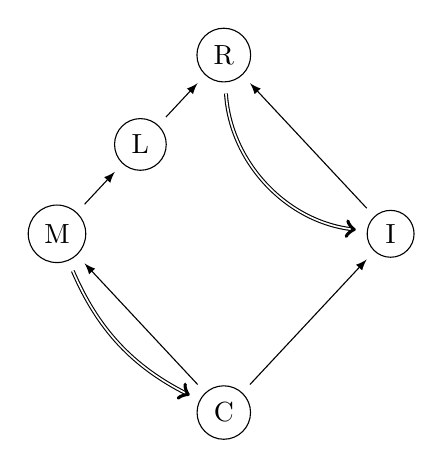
\begin{tikzpicture}[shorten <=0.4em,shorten >=0.4em]
\node [circle,draw,shift={(1ex,15ex)}] (M){M};
\node [circle,draw,shift={(15ex,0ex)}] (C){C};
\node [circle,draw,shift={(29ex,15ex)}] (I){I};
\node [circle,draw,shift={(8ex,22.5ex)}] (L){L};
\node [circle,draw,shift={(15ex,30ex)}] (R){R};
\draw [arrows={-latex}] (I) -- (R);
\draw [arrows={-latex}] (M) -- (L);
\draw [arrows={-latex}] (L) -- (R);
\draw [arrows={-latex}] (C) -- (M);
\draw [arrows={-latex}] (C) -- (I);
\draw[->,double] (M) to[bend right=20] (C);
\draw[->,double](R) to[bend right=40] (I); 
\end{tikzpicture}
\end{Scaled}
\end{minipage}
\begin{minipage}[H]{0.5\textwidth}
\begin{Scaled}{0.6}{0.6}
$
\begin{array}{|l}
\mbox{Nodes:}
\\
\begin{array}{l l}

\begin{tikzpicture}[shorten <=0.4em,shorten >=0.4em]
\node [circle,draw,shift={(0,0)}] (M){M};
\end{tikzpicture}
&\raisebox{1.5ex}{Mutable: alias, write}
\\
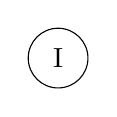
\begin{tikzpicture}[shorten <=0.4em,shorten >=0.4em]
\node [circle,draw,shift={(0,0)}] (I){${\ }$I${\ }$ };
\end{tikzpicture}
&\raisebox{1.5ex}{Immutable: alias, no write}
\\

\begin{tikzpicture}[shorten <=0.4em,shorten >=0.4em]
\node [circle,draw,shift={(0,0)}] (C){C};
\end{tikzpicture}
&\parbox{50ex}{Capsule: unique access\\*
Reference used only once}
\\

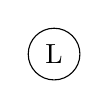
\begin{tikzpicture}[shorten <=0.4em,shorten >=0.4em]
\node [circle,draw,shift={(0,0)}] (L){L};
\end{tikzpicture}
&
\parbox{50ex}{Lent: no alias, write}
\\

\begin{tikzpicture}[shorten <=0.4em,shorten >=0.4em]
\node [circle,draw,shift={(0,0)}] (C){R};
\end{tikzpicture}
&
\parbox{50ex}{Readable: no alias, no write}
\end{array}
\\
\mbox{Arrows:}
\\
\begin{array}{l l}
\begin{tikzpicture}
\draw [arrows={-latex}] (0,0) -- (1,0);
\end{tikzpicture}
&\mbox{Subtype}
\\
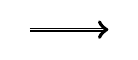
\begin{tikzpicture}
\draw[->,double] (0,0) to (1,0);
\end{tikzpicture}
&\mbox{{Recovery}}
\end{array}
\end{array}
$
\end{Scaled}
\end{minipage}
}
\caption{Type qualifiers and their relationships}
\label{fig:hierarchy}
\end{figure}

\section{Type system}\label{sect:typesystem}
Type contexts are defined by:
\begin{center}
\begin{grammatica}
\produzione{\Delta}{\Gamma;\LentLocked;\StronglyLocked}{type context}\\*
\produzione{\Gamma}{\TypeDec{\T_1}{\x_1},\ldots,\TypeDec{\T_n}{\x_n}}{type assignment}
\end{grammatica}
\end{center} 
{In a type context $\Delta=\Gamma;\LentLocked;\StronglyLocked$, $\Gamma$ is a usual {\em assignment of types} to variables. We write $\dom{\Gamma}$ for the set of variables in $\Gamma$, and  $\SubstFun{\Gamma}{\Gamma'}$ for the concatenation of $\Gamma$ and $\Gamma'$ where, for the variables occurring in both domains, $\Gamma'$ takes precedence.  We will also use $\domMut{\Gamma}$ for the set of mutable variables in $\Gamma$, and other analogous notations.}

{According to our convention, $\LentLocked$ is a sequence $\xs_1\ldots\xs_n$ of sequences of variables, and $\StronglyLocked$ is a sequence of variables. All such sequences are assumed to be sets (that is, order and repetitions are immaterial). The sets  $\xs_1\ldots\xs_n$ are assumed to be pairwise disjoint, and are called \emph{{lent group}s}, whereas the $\mutable$ variables in $\Gamma$ which do not belong to any lent group form the \emph{{mutable group}}. Finally, variables in $\ys$ are called \emph{restricted} variables.}

{Lent groups and restricted variables are the key novelty of our type system.
%, hence we roughly explain their role, which will be formally detailed in the following. 
The property they ensure is that, if $\TypeCheck{\Gamma}{\LentLocked}{\StronglyLocked}{\e}{\T}$, then the final result of $\e$ will be not connected to variables which are in $\LentLocked$ or $\StronglyLocked$. In this way, to ensure that the final result of $\e$ is an isolated portion of store, it is enough to typecheck $\e$ in a type context where all its free mutable variables are in a {lent group} or restricted.  This is a crucial improvement with respect to previous mechanisms of recovery \cite{GordonEtAl12,ClebschEtAl15}, where this could be only ensured if  $\e$ had \emph{only} immutable or isolated ($\capsule$ in our teminology) free variables. 
We have distinct {lent group}s $\xs_1\ldots\xs_n$ since there can be nested recoveries, hence, to ensure that all are safe, we need also the auxiliary property that no aliasing is introduced between different groups, as will be illustrated in detail by the last example of \refToSection{examples}. That is, if the reachable graphs of $\xs_i$ and $\xs_j$ were disjoint before the evaluation of the expression, then after the evaluation they should be still disjoint.\footnote{Note that this is different from \emph{regions} as in, e.g., \cite{BocchinoEtAl09,HallerOdersky10}, which are sets of references \emph{assumed} to be disjoint.}} 

{The type system ensures the above properties by imposing that variables in $\LentLocked$ and $\StronglyLocked$ are used in controlled way:
\begin{itemize}
\item A $\mutable$ variable in $\Gamma$ which belongs to a {lent group} $\xs_i$ can only be used as $\lent$. Notably, write access is not directly allowed since it could introduce aliasing.
\item A $\readable$, $\lent$ or $\mutable$ variable in $\Gamma$ which is restricted cannot be used at all, that is, is hidden.\footnote{{However, we use the terminology ``restricted'' since this hiding is non permanent.}}
\end{itemize}
The important point is that such constraints are not imposed once and for all when typechecking an expression. That is, a subexpression can be typechecked with different {lent group}s and restricted variables, more precisely:
\begin{itemize}
\item In a subexpression we can \emph{swap} one of the {lent group}s $\xs_i$ with the {mutable group}, weakening to $\lent$ the type of the subexpression if it was mutable. 
In this way, write access to variables in $\xs_i$ is allowed, but this is safe since the result of the subexpression is in turn $\lent$, so no aliasing can be introduced with the result of the main expression. 
\item In a subexpression we can \emph{unrestrict} variables in $\ys$, that is, freely use such variables, provided that the type of the subexpression is $\imm$ or $\capsule$.  Again this guarantees that no aliasing can be introduced with the result of the main expression.
\end{itemize} }

Lent groups and restricted variables are introduced as an effect of applying \emph{recovery} rules \rn{t-capsule} and \rn{t-imm}, whereas swapping and unrestricting are obtained by applying rules \rn{{t-swap}} and \rn{t-unrst} rules, as will be explained in detail later. 


Contexts $\Delta=\Gamma;\LentLocked;\StronglyLocked$ are \emph{well-formed}, written $\WellFormedTypeCtx{\Delta}$, 
if, for $\LentLocked=\xs_1\ldots\xs_n$, the following conditions hold:
\begin{itemize}
\item no variable is $\lent$  in $\Gamma$
\item if  $\x\in\xs_i$ for some $i\in 1..n$,  then $\x$ is $\mutable$ in $\Gamma$
\item if $\y\in\StronglyLocked$, then  $\y$ is $\mutable$ or $\readable$  in $\Gamma$
\item if $\y\in\StronglyLocked$ and is $\mutable$ in $\Gamma$, then $\y\in\xs_i$ for some $i\in 1..n$.
%and, for all $\x\in\xs_i$, $\x\in\StronglyLocked$
\end{itemize}
We do not consider $\lent$ variables in $\Gamma$ since assigning the type $\Type{\lent}{\C}$ to a variable $\x$  is encoded by assigning to $\x$ the type $\Type{\mutable}{\C}$ and having $\x$ in a lent group in $\LentLocked$ (see the explanation of rule \rn{t-block} in the following). The  last condition requires \emph{coherency} between $\LentLocked$ and $\StronglyLocked$, that is, restricted mutable variable are in a lent group. It is easy to check that well-formedness of contexts is preserved in type derivations. That is, if $\Delta\TypeCheckGround{\e}{\T}$ and ${\Delta}$ is well-formed, then in all sub-derivations the contexts are well-formed. In the following when we write 
$\Delta\TypeCheckGround{\e}{\T}$ we assume that ${\Delta}$ is well-formed.

In the rules we use information extracted from the class table, which is modelled, as usual, by the following functions:{
\begin{itemize}
\item $\fields{\C}$ gives, for each declared class $\C$, the sequence of its fields declarations
\item {$\method{\C}{\m}$ gives, for each method $\m$ declared in class $\C$, the tuple\\
 $\FourTuple{\T}{\mu}{\Param{\T_1}{\x_1}\ldots\Param{\T_n}{\x_n}}{\e}$ consisting of its return type, type qualifier for $\this$, parameters, and body. }
\end{itemize}
We assume method bodies to be well-typed w.r.t.\ {the type annotations in the method declaration}. More precisely, if
%\begin{quote}
%$\method{\C}{\m}=\FourTuple{\T}{\mu}{\Param{\T_1}{\x_1}\ldots\Param{\T_n}{\x_n}}{\e}$
%\end{quote}
%then $\e$ should be well-typed in a type context where parameters declared $\lent$, including the implicit parameter $\this$, have been encoded by singleton lent groups, expressing the requirement that they should not be aliased by the method. Formally, it should be
%\begin{quote}
%$\TypeCheck{\Gamma}{\{\x_i\mid T_i=\Type{\lent}{\C_i}\}\cup\{\this\mid\mu=\lent\}}{\emptyset}{\e}{\T}$
%\end{quote}
%with $\Gamma=\TypeDec{\Type{\mu'}{\C}}{\this}, \TypeDec{\T'_1}{\x_1},\ldots,\TypeDec{\T'_n}{\x_n}$, where $\T_i=\Type{\mutable}{\C_i}$ if $\T_i=\Type{\lent}{\C_i}$, $\T'_i=\T_i$ otherwise, and $\mu'=\mutable$ if $\mu=\lent$, $\mu'=\mu$ otherwise. 
{\begin{quote}
$\method{\C}{\m}=\FourTuple{\T}{\mu}{\Param{\T_1}{\x_1}\ldots\Param{\T_n}{\x_n}}{\e}$
\end{quote}
then 
\begin{quote}
$\TypeCheck{\Gamma}{\LentLocked}{\emptyset}{\e}{\T}$
\end{quote}
where $\LentLocked$ {consists of} the singletons of the parameters declared $\lent$, including the implicit parameter $\this$, expressing the requirement that they should not be aliased by the method, and $\Gamma=\TypeDec{\Type{\mu'}{\C}}{\this}, \TypeDec{\T'_1}{\x_1},\ldots,\TypeDec{\T'_n}{\x_n}$, where $\T_i=\Type{\mutable}{\C_i}$ if $\T_i=\Type{\lent}{\C_i}$, $\T'_i=\T_i$ otherwise, and $\mu'=\mutable$ if $\mu=\lent$, $\mu'=\mu$ otherwise. 
}

Typing rules are given in \refToFigure{typing}. {In the typing rules, when we need to make explicit the mutable group, we use the  auxiliary judgment $\AuxTypeCheck{\Gamma}{\LentLocked}{\MutGroup}{\StronglyLocked}{\e}{\T}$, which stands for the judgment 
$\TypeCheck{\Gamma}{\LentLocked}{\StronglyLocked}{\e}{\T}$ with the side condition $\MutGroup=\domMut{\Gamma}{\setminus}\LentLocked$, meaning that $\MutGroup$ are the $\mutable$ variables in $\Gamma$ which do not belong to {any lent} group in $\LentLocked$.}

\begin{figure}[ht!]
\framebox{
\begin{footnotesize}
\begin{math}
\begin{array}{l}
\NamedRule{t-capsule}{\AuxTypeCheck{\Gamma}{\LentLocked\ {\xs}}{{\emptyset}}{\StronglyLocked}{\e}{\Type{\mutable}{\C}}}{{\AuxTypeCheck{\Gamma}{\LentLocked}{\MutGroup}{\StronglyLocked}{\e}{\Type{\capsule}{\C}}}}\\
\Space
%{\xs=\domMut{\Gamma}{\setminus}\LentLocked}
\NamedRule{t-imm}{
\AuxTypeCheck{\Gamma}{\LentLocked\ \xs}{{\emptyset}}{\domGeqMut(\Gamma) }{\e}{\Type{\readable}{\C}}
}{
{\AuxTypeCheck{\Gamma}{\LentLocked}{\xs}{\StronglyLocked}{\e}{\Type{\imm}{\C}}}
}{
%{\xs=\domMut{\Gamma}{\setminus}\LentLocked}
}
\\[5ex]
\NamedRule{{t-swap}}{\AuxTypeCheck{\Gamma}{\LentLocked\ \xs'}{\xs}{\StronglyLocked}{\e}{{\T}}}{{\AuxTypeCheck{\Gamma}{\LentLocked\ \xs}{\xs'}{\StronglyLocked}{\e}{{\TPrime}}}}{
%{\xs'=\domMut{\Gamma}{\setminus}(\LentLocked\ \xs)}\\
{\xs\cap\ys}=\emptyset\\
{\TPrime=
\begin{cases}
\Type{\lent}{\C}&\mbox{if}\ \T=\Type{\mutable}{\C}\\
\T&\mbox{otherwise}
\end{cases}}
}
\\[5ex]
\NamedRule{t-{unrst}}{
\TypeCheck{\Gamma}{\LentLocked}{\emptyset}{\e}{{\T}}
}{
\TypeCheck{\Gamma}{\LentLocked}{\StronglyLocked}{\e}{{\T}}
}{{\T=\Type{\mu}{\C}\Longrightarrow\mu\leq\imm}}
\Space
\NamedRule{t-sub}{\TypeCheckShort{\Delta}{\e}{\T}
}{
\TypeCheckShort{\Delta}{\e}{\TPrime}}{
\T\leq\TPrime
}
\\[5ex]
{\NamedRule{t-var}{}{\TypeCheck{\Gamma}{\LentLocked}{\StronglyLocked}{\x}{\TPrime}}{
\Gamma(\x)=\T\ \wedge \ 
\x\notin\StronglyLocked\\
\TPrime=
\begin{cases}
\Type{\lent}{\C}&\mbox{if}\ \T{=}\Type{\mutable}{\C}\,\wedge\,\x\in\LentLocked\\
\T&\mbox{otherwise}
\end{cases}
}}
\\[6ex]
{\NamedRule{t-field-access}{\TypeCheckShort{\Delta}{\e}{\Type{\mu}{\C}}}{\TypeCheckShort{\Delta}{\FieldAccess{\e}{\f_i}}{\TPrime_i}}{
\fields{\C}=\Field{\T_1}{\f_1}\ldots\Field{\T_n}{\f_n}\\
\TPrime_i=\begin{cases}
\Type{\mu}{\C_i}\ \mbox{if}\ \T_i=\Type{\mutable}{\C_i}\\
\T_i\ \mbox{otherwise}
\end{cases}
}}
\\[5ex]
\NamedRule{t-meth-call}{\TypeCheckShort{\Delta}{\e_i}{\T_i}\Space\forall i\in 0..n}{\TypeCheckShort{\Delta}{\MethCall{\e_0}{\m}{\e_1,\ldots,\e_n}}{\T}}{
\begin{array}{l}
\T_0=\Type\mu\C\\
\method{\C}{\m}=\FourTuple{\T}{\mu}{\Param{\T_1}{\x_1}\ldots\Param{\T_n}{\x_n}}{\e}
\end{array}
}
\\[5ex]
\NamedRule{t-field-assign}{
  \TypeCheckShort{\Delta}{\e}{\Type{\mutable}{\C}}
  \Space
  \TypeCheckShort{\Delta}{\e'}{\T_i}
  }{
  \TypeCheckShort{\Delta}{\FieldAssign{\e}{\f_i}{\e'}
  }{\T_i}
  }{
  {\fields{\C}=\Field{\T_1}{\f_1}\ldots\Field{\T_n}{\f_n}}
  }
\\[5ex]
\NamedRule{t-new}{\TypeCheckShort{\Delta}{\e_i}{\T_i}\Space\forall i\in 1..n}{\TypeCheckShort{\Delta}{\ConstrCall{\C}{\e_1,\ldots,\e_n}}{\Type{\mutable}{\C}}}{
\fields{\C}=\Field{\T_1}{\f_1}\ldots\Field{\T_n}{\f_n}\\
}
\\[5ex]
{\NamedRule{t-block}{
{\AuxTypeCheck{\SubstFun{\Gamma}{\TypeEnv{\decs}}}{\LentLocked_i}{\MutGroup_i}{\StronglyLocked'}{\e_i}{\TypeEnv{\decs}(\x_i)}\ \ {\forall i\in 1..n}}\\
\AuxTypeCheck{\SubstFun{\Gamma}{\TypeEnv{\decs}}}{\LentLocked'}{{\MutGroup'}}{\StronglyLocked'}{\e}{\T}}
{\AuxTypeCheck{\Gamma}{\LentLocked}{\MutGroup}{\StronglyLocked}{\Block{\decs}{\e}}{\T}}{
\begin{array}{l}
\decs=\Dec{\T_1}{\x_1}{\e_1}\ldots\Dec{\T_n}{\x_n}{\e_n}\\
\LessEq{(\LentLocked{\setminus}\dom{\decs})}{\LentLocked'}\\
(\MutGroup{\setminus}\dom{\decs})\subseteq\MutGroup'\\
\forall i\in 1..n\ \LentLocked_i\ \MutGroup_i = \LentLocked'\ \MutGroup'\\
\Space \mbox{and}\ \x_i\in\domMut{\TypeEnv{\decs}}\Rightarrow\x_i\in \MutGroup_i\\
\StronglyLocked'={\StronglyLocked}{\setminus}{\dom{\decs}}
\end{array}}}
\end{array}
\end{math}
\end{footnotesize}
}
\caption{Typing rules}\label{fig:typing}
\end{figure}
 
Rules \rn{t-{capsule}} and \rn{t-{imm}} 
 model \emph{recovery},
 that is, can be used to recover a more specific type for an expression,
 under the conditions that the use of some free variables in the expression is} {controlled}.
There are two kinds of recovery:
\begin{itemize}
\item $\mutable\Rightarrow\capsule$
\\* As shown in rule \rn{t-{capsule}}, an expression can be typed $\capsule$ in $\Gamma;\LentLocked;\StronglyLocked$ if it can be typed $\mutable$ by turning in lent the mutable group ($\xs$), which becomes empty.
Formally, this group is added to $\LentLocked$.  
\item $\readable\Rightarrow\imm$ 
\\*As shown in rule \rn{t-{imm}}, an expression can be typed $\imm$ in $\Gamma;\LentLocked;\StronglyLocked$  if it can be typed $\readable$ by {turning in lent the mutable group ($\xs$)}, as in the {recovery} above, and, moreover, restricting currently available mutable, lent, and readable variables ($\domGeqMut(\Gamma)$).
\end{itemize}

Along with {recovery} rules which introduce {lent group}s and restricted variables, we have two corresponding elimination rules.
In the detail:
\begin{itemize}
\item\rn{{t-swap}}
\\* An expression can be typed in $\Gamma;\LentLocked\ \xs;\StronglyLocked$ if it can be typed by turning into mutable 
some {lent group} {($\xs$)}, by swapping this group with the {current mutable group}  ($\xs'$). {The side condition $\xs\cap\ys=\emptyset$ prevents to swap a lent group including restricted variables.}
The type obtained in this way is weakened to $\lent$, if it was $\mutable$.
\item
\rn{t-unrst} 
\\* An expression can be typed in $\Gamma;\LentLocked;\StronglyLocked$ if it can be typed by unrestricting all restricted variables {$\StronglyLocked$}, provided that the type obtained in this way is $\capsule$ or $\imm$ {or a primitive type}.
\end{itemize}

{Note that, without these last two rules, recovery rules would be essentially equivalent to those in prior work \cite{GordonEtAl12,ClebschEtAl15}. Rules \rn{t-swap} and \rn{t-unrst}  add power to the type system, and they are also the reason {it} requires the $\LentLocked$ and $\StronglyLocked$ information during typechecking.
Prior work \cite{GordonEtAl12,ClebschEtAl15} can afford to simply locally using weakening and subtyping to make references inaccessible
or convert $\mutable$ references to $\lent$.}

{Note also that recovery rules, \rn{t-swap}, and \rn{t-unrst}  are not syntax-directed, analogously to the subsumption rule. 
In other words, their functionality does not  restrict how code is written: they are \emph{transparent} to the programmer, in the sense that they are applied when needed.  The programmer can simply rely on the fact that expressions are $\capsule$ or $\imm$, respectively, in situations where this is intuitively expected, as we illustrate by the following examples (other will be provided in next section).}

{We explain now in detail how recovery, swapping and unrestricting work, then comment the other rules.}

\paragraph{Capsule {recovery}} Let us discuss, first, when an expression can be safely typed $\capsule$. {The evaluation of the expression should produce a portion of store which is isolated, apart from external immutable references, formally a right-value where all free variables are immutable. Obviously, this is safe for an expression which has itself no free variables, or where all the free variables are {$\imm$ or $\capsule$}, and, indeed, this was the requirement needed for obtaining {recovery} in previous work \cite{GordonEtAl12}.} However, this requirement is too strong. 
Consider the following sequence of declarations:\label{capsule-example-2}

\begin{lstlisting}
mut D y=new D(0); 
capsule C z={mut D x=new D(y.f); new C(x,x)};  
\end{lstlisting}

The inner block (right-hand side of the declaration of \Q@z@) {can} be typed $\capsule$, even though there is a mutable free variable \Q@y@, since this variable is only used in a field access, hence, intuitively, no aliasing is introduced between \lstinline{y}{} and the final result of the block. 
Indeed, the block reduces\footnote{As formalized in \refToSection{calculus}.} to 
\begin{lstlisting} 
{mut D x=new D(0); new C(x,x)};  
\end{lstlisting}
which is closed.
%, that is, has no free variables. 
To allow such typing, the inner block is {typed} applying rule \rn{t-capsule}, since it can be typechecked $\mutable$ in a type context where variable \lstinline{y}{} is $\lent$. In \refToFigure{TypingOne} we show the type derivation for this example,
{where, for clarity, we always write the mutable group even when it is empty.}
%We use $\deriv$ as a metavariable to denote derivations.
\begin{figure}[t]
\framebox{
\begin{footnotesize}
\begin{math}
\begin{array}{l}
\\
\infer[\scriptstyle{\textsc{(t-capsule)}}]
{\TypeCheck{\Gamma}{\emptyset\ [\texttt{y}]}{\emptyset}{\texttt{\{mut D x=new D(y.f); new C(x,x)\}}}{\Type{\capsule}{\C}}}
{
\infer[\scriptstyle{\textsc{(t-block)}}]
{\TypeCheck{\Gamma}{\texttt{y}\ [\emptyset]}{\emptyset}{\texttt{\{mut D x=new D(y.f); new C(x,x)\}}}{\Type{\mutable}{\C}}}
{
%\infer[\scriptstyle{\textsc{(t-sub)}}]
%{ \TypeCheck{\Gamma'}{\texttt{y}}{\emptyset}{\texttt{new D(y.f)}}{\Type{\lent}{\texttt{D}}}      }
{
\infer[\scriptstyle{\textsc{(t-new)}}]
{\TypeCheck{\Gamma'}{\texttt{y}\ [\texttt{x}]}{\emptyset}{\texttt{new D(y.f)}}{\Type{\mutable}{\texttt{D}}}}
{
\infer[\scriptstyle{\textsc{(t-field-access)}}]
{\TypeCheck{\Gamma'}{\texttt{y}\ [\texttt{x}]}{\emptyset}{\texttt{y.f}}{\intType}}
{
\infer[\scriptstyle{\textsc{(T-var)}}]
{\TypeCheck{\Gamma'}{\texttt{y}\ [\texttt{x}]}{\emptyset}{\texttt{y}}{\Type{\lent}{\texttt{D}}}}{} 
}
}
}
&
\infer[\scriptstyle{\textsc{(T-New)}}]
{\TypeCheck{\Gamma'}{\texttt{y}\ [\texttt{x}]}{\emptyset}{\texttt{new C(x,x)}}{\Type{\mutable}{\texttt{C}}}}
{
\infer[\scriptstyle{\textsc{(T-var)}}]
{\TypeCheck{\Gamma'}{\texttt{y}\ [\texttt{x}]}{\emptyset}{\texttt{x}}{\Type{\mutable}{\texttt{D}}}}
{} 
}
}
}
\\
\\
\Gamma=\texttt{y}{:}\Type{\mutable}{\texttt{D}},\texttt{z}{:}\Type{\capsule}{\texttt{C}}\\
\Gamma'=\SubstFun{\Gamma}{\texttt{x}{:}\Type{\mutable}{\texttt{D}}}=\texttt{y}{:}\Type{\mutable}{\texttt{D}},\texttt{z}{:}\Type{\capsule}{\texttt{C}},\texttt{x}{:}\Type{\mutable}{\texttt{D}}
\end{array}
\end{math}
\end{footnotesize}
}
\caption{Example of type derivation (1)}\label{fig:TypingOne}
\end{figure}

{Note that in an analogous example where the field of class \lstinline{D} has a non primitive type, e.g., \lstinline{String}:}
\begin{lstlisting}
mut D y=new D("hello"); 
capsule C z={mut D x=new D(y.f); new C(x,x)};  
\end{lstlisting}
{the qualifier of the field should be $\imm$, since, otherwise, by introducing a singleton {lent group} \lstinline{y} we would get a $\lent$ type for \lstinline{y.f} as well, see rule \rn{t-field-access}, and a $\lent$ type is not accepted for a constructor argument.}

As a counterexample, consider the following sequence of declarations:
\begin{lstlisting}
mut D y=new D(0); 
capsule C z={mut D x=y; new C(x,x)};  
\end{lstlisting}
Here the inner block cannot be typed $\capsule$, since \Q@y@ is internally aliased. Indeed, the block reduces to \Q@new C(y,y)@ which contains a free mutable variable.
Formally, we cannot apply rule \rn{t-capsule} on the block, since
we should typecheck the block with \Q@y@ in a singleton {lent group}, while the initialization expression of \lstinline{x} should be mutable, see rule \rn{t-block}.

Rule \rn{t-field-assign} requires a mutable type for the receiver.
So, how is it possible to modify (the portion of store denoted by) a $\lent$ reference?
Consider the following simple example:
\begin{lstlisting}
lent D y= new D(0);
y.f=y.f+1;
\end{lstlisting}

This code should be well-typed, since the assignment does not introduce any alias. {To get such typing, we use rule \rn{t-swap} to type the expression
\Q@y.f=y.f+1@. {Indeed, we can} swap the singleton {lent group} \Q@y@ with the empty set.

Moreover, swapping can be applied to achieve {recovery}. Take
the example already considered at page \pageref{capsule-example-1}:
\begin{lstlisting}
mut D y=new D(0); 
capsule C z={mut D x=new D(y.f=y.f+1); new C(x,x)}
\end{lstlisting}
Let $\e$ be the inner block (right-hand side of the declaration of \Q@z@). As in the first example, $\e$ can be typed $\capsule$ if it can be typed \Q@mut@ in a context with type assignment $\texttt{y}{:}\Type{\mutable}{\texttt{D}},\texttt{z}{:}\Type{\capsule}{\texttt{C}}$ and
the {lent group} \Q@y@. However, the assignment \Q@y.f=y.f+1@
is not well-typed in this type context, since the variable \Q@y@ has type \Q@lent D@. However, intuitively, we can see that the assignment does not introduce any alias between \Q@y@ and the final result of $\e$, since it involves only variables which are in the same group (the
singleton \Q@y@), and produces {a result which is not mutable}. {In other words, the result of the evaluation of $\e$ is a capsule, as it has been shown in \refToFigure{esRed2}, so it should be possible to
{type} the expression $\e$ {as} $\capsule$.} 

To {get} such typing, we can apply rule \rn{t-swap} when deriving the type for the subexpression \Q@y.f=y.f+1@, by swapping the group \Q@y@ with the group \Q@x@. 
This ensures that the evaluation of the subexpression typed by this rule will not introduce any alias between the
variables in the swapped group and the mutable group. {The type derivation for the example is given in \refToFigure{TypingTwo}.}
 \begin{figure}[t]
 \framebox{
\begin{footnotesize}
\begin{math}
\begin{array}{l}
\infer[\scriptstyle{\textsc{(t-capsule)}}]
{\TypeCheck{\Gamma}{\emptyset\ [\texttt{y}]}{\emptyset}{\texttt{\{mut D x=new D(y.f=y.f+1); new C(x,x)\}}}{\Type{\capsule}{\texttt{C}}}}
{
\infer[\scriptstyle{\textsc{(t-block)}}]
{\TypeCheck{\Gamma}{\texttt{y}\ [\emptyset]}{\emptyset}{\texttt{\{mut D x=new D(y.f=y.f+1); new C(x,x)\}}}{\Type{\mutable}{\texttt{C}}}
}
{
\infer[\scriptstyle{\textsc{(T-New)}}]
{\TypeCheck{\Gamma'}{\texttt{y}\ [\texttt{x}]}{\emptyset}{\texttt{new C(x,x)}}{\Type{\mutable}{\texttt{C}}}}
{
\infer[\scriptstyle{\textsc{(T-var)}}]
{\TypeCheck{\Gamma'}{\texttt{y}\ [\texttt{x}]}{\emptyset}{\texttt{x}}{\Type{\mutable}{\texttt{D}}}}{}
}
&
\hspace{-1cm}
\infer[\scriptstyle{\textsc{(T-New)}}]
{\TypeCheck{\Gamma'}{\texttt{y}\ [\texttt{x}]}{\emptyset}{\texttt{new D(y.f=y.f+1)}}{\Type{\mutable}{\texttt{D}}}}
{
\infer[\scriptstyle{\textsc{(t-swap)}}]
{\TypeCheck{\Gamma'}{\texttt{y}\ [\texttt{x}]}{\emptyset}{\texttt{y.f=y.f+1}}{\intType}}
{
\infer[\scriptstyle{\textsc{(t-fld-ass)}}]
{\TypeCheck{\Gamma'}{\texttt{x}\ [\texttt{y}]}{\emptyset}{\texttt{y.f=y.f+1}}{\intType}}
{
\infer[\scriptstyle{\textsc{(T-var)}}]
{\TypeCheck{\Gamma'}{\texttt{x}\ [\texttt{y}]}{\emptyset}{\texttt{y}}{\Type{\mutable}{\texttt{D}}}}{}
&
\deduce{\TypeCheck{\Gamma'}{\texttt{x}\ [\texttt{y}]}{\emptyset}{\texttt{y.f+1}}{\intType}}{\vdots}
}
}
}
}
}\\
\\
\Gamma=\texttt{y}{:}\Type{\mutable}{\texttt{D}},\texttt{z}{:}\Type{\capsule}{\texttt{C}}\\
\Gamma'=\SubstFun{\Gamma}{\texttt{x}{:}\Type{\mutable}{\texttt{D}}}=\texttt{y}{:}\Type{\mutable}{\texttt{D}},\texttt{z}{:}\Type{\capsule}{\texttt{C}},\texttt{x}{:}\Type{\mutable}{\texttt{D}}
\end{array}
\end{math}
\end{footnotesize}
}
\caption{Example of type derivation (2)}\label{fig:TypingTwo}
\end{figure}

Note that, when using rule \rn{t-swap} to typecheck a subexpression of an expression {for which we want the capsule or immutability property}, no alias should be introduced between the variables in the group $\xs$ and the result of the expression.  Indeed, in this case the result of the subexpression could contain references to the variables in group $\xs$, which was lent in the original context.To ensure this, the type obtained in this way is weakened to $\lent$, if it was $\mutable$. 
 This is shown by the following example:
\begin{lstlisting}
mut D y=new D(x1,x2);  
mut x1=new A(0); 
mut x2=new A(1);
capsule C z={mut A x=(y.f1=y.f2); new C(x,x)};
\end{lstlisting}
If we apply rule \rn{{t-swap}} when deriving the
type for \Q@y.f1=y.f2@, therefore swapping the group \Q@y@ with \Q@x@, then we derive type
\Q@mut A@, and rule \rn{{t-swap}} would assign type \Q@lent A@ to the expression.
Therefore, the declaration \Q@mut A x=(y.f1=y.f2)@ and the whole expression would be ill-typed.
Indeed, the expression reduces to
\begin{lstlisting}
mut D y=new D(x2,x2);  
mut x1=new A(0); 
mut x2=new A(1);
capsule C z=new C(x2,x2);
\end{lstlisting}
in which the value of \Q@z@ is not a capsule.

\paragraph{{Immutability recovery}} 
{Note that $\capsule$ recovery can only happen for $\mutable$ expressions. In other words, $\mutable$ expressions which reduce to a portion of store with no external mutable references can be safely used where (either a mutable or) an immutable is required. Indeed, every expression which can be typed $\capsule$ can be typed $\imm$ by subtyping. }

{Consider now an expression for which $\capsule$ recovery cannot happen, that is, which can be typed $\lent$ or $\readable$, but cannot be typed $\mutable$, hence should not be used where a $\mutable$ is required. We can \emph{directly}\footnote{That is, not by subtyping.} recover immutability for such an expression, if we can guarantee that the result of the expression will be not connected to external mutable references.   This can be ensured as for the case of $\capsule$ recovery, with one difference. For $\capsule$ recovery, $\lent$ and $\readable$ references can be freely used, since in any case they will be not connected to the final result of the expression. However, if the expression is in turn $\lent$ or $\readable$, its result \emph{could} be connected to $\lent$ or $\readable$ references, hence this should be explicitly prevented by the type system. This is achieved by \emph{restricting} such references, that is, allowing their use only to typecheck subexpressions of $\imm$ $\capsule$ or primitive type.}

Consider the following variant of the first example of capsule {recovery}:
\begin{lstlisting}
mut D y=new D(0); 
imm C z={lent D x=new D(y.f); new C(x,x)};  
\end{lstlisting}
As in the original version, the inner block (right-hand side of the declaration of \lstinline{z}) uses the mutable free variable \lstinline{y} only in a field access, and indeed reduces to the block \Q@{lent D x= new D(0);  new C(x,x)}@ which is closed. However, this block {cannot be typed $\capsule$}, since it cannot be safely assigned to a mutable reference. On the other hand, the block can be safely typed  $\imm$, since, intuitively, it reduces to a portion of store which cannot be modified through any other reference. Formally, the inner block can be {typed $\imm$} by rule \rn{t-imm}, since it can be typechecked $\lent$ in a type context where variable \lstinline{y}{} is in  singleton {lent group} and, moreover, restricted, that is, can be only used to typecheck subexpressions which are $\imm$, $\capsule$, or of a primitive type. 
The type derivation for the example is given in \refToFigure{TypingThree}. 
{Note that, instead of putting \texttt{x} is a sigleton group we could have put \texttt{x} and \texttt{y} in the same 
group in the typing of \lstinline{new C(x,x)}{} and \lstinline{new D(y.f)}{}. That is, replacing}
\verb!{x} {y}! with \verb!{x,y}!  the derivation would still be correct. (Clearly the rule \rn{T-Swap} would swap \verb!{x,y}!
with the empty mutable group.)

\begin{figure}[th]
\framebox{
\begin{footnotesize}
\begin{math}
\begin{array}{l}
\\
\infer[\scriptstyle{\textsc{(t-imm)}}]
{\TypeCheck{\Gamma}{\emptyset\ [\texttt{y}]}{\emptyset}{\texttt{\{lent D x=new D(y.f); new C(x,x)\}}}{\Type{\imm}{\texttt{C}}}}
{
\infer[\scriptstyle{\textsc{(t-block)}}]
{\TypeCheck{\Gamma}{\texttt{y}\ [\emptyset]}{\texttt{y}}{\texttt{\{lent D x=new D(y.f); new C(x,x)\}}}{\Type{\lent}{\texttt{C}}}
}
{
\infer[\scriptstyle{\textsc{(t-new)}}]
{
\TypeCheck{\Gamma'}{\{\texttt{y}\}\ \{\texttt{x}\}\ [\emptyset]}{\texttt{y}}{\texttt{new D(y.f)}}{\Type{\mutable}{\texttt{D}}}
}
{
\infer[\scriptstyle{\textsc{(t-unrst)}}]
{\TypeCheck{\Gamma'}{\{\texttt{y}\}\ \{\texttt{x}\}\ [\emptyset]}{\texttt{y}}{\texttt{y.f}}{\intType}}
{
\infer[\scriptstyle{\textsc{(t-field-access)}}]
{\TypeCheck{\Gamma'}{\{\texttt{y}\}\ \{\texttt{x}\}\ [\emptyset]}{\emptyset}{\texttt{y.f}}{\intType}}
{
\infer[\scriptstyle{\textsc{(T-var)}}]
{\TypeCheck{\Gamma'}{\{\texttt{y}\}\ \{\texttt{x}\}\ [\emptyset]}{\emptyset}{\texttt{y}}{\Type{\lent}{\texttt{D}}}}{} 
}
}
}
&
\infer[\scriptstyle{\textsc{(t-swap)}}]
{\TypeCheck{\Gamma'}{\{\texttt{y}\}\ \{\texttt{x}\}\ [\emptyset]}{\texttt{y}}{\texttt{new C(x,x)}}{\Type{\lent}{\texttt{C}}}}
{
\infer[\scriptstyle{\textsc{(t-new)}}]
{\TypeCheck{\Gamma'}{\texttt{y}\ [\texttt{x}]}{\texttt{y}}{\texttt{new C(x,x)}}{\Type{\mutable}{\texttt{C}}}}
{
\infer[\scriptstyle{\textsc{(T-var)}}]
{\TypeCheck{\Gamma'}{\texttt{y}\ [\texttt{x}]}{\texttt{y}}{\texttt{x}}{\Type{\mutable}{\texttt{D}}}}{}
}
}
}
}
\\  \\
\Gamma=\texttt{y}{:}\Type{\mutable}{\texttt{D}},\texttt{z}{:}\Type{\imm}{\texttt{C}}\\
\Gamma'=\SubstFun{\Gamma}{\texttt{x}{:}\Type{\mutable}{\texttt{D}}}=\texttt{y}{:}\Type{\mutable}{\texttt{D}},\texttt{z}{:}\Type{\imm}{\texttt{C}},\texttt{x}{:}\Type{\mutable}{\texttt{D}}
\end{array}
\end{math}
\end{footnotesize}
}
\caption{Example of type derivation (3)}\label{fig:TypingThree}
\end{figure}

{Restricting $\y$} prevents typechecking examples like the following:
\begin{lstlisting}
mut D y=new D(0); 
imm C z={lent D x=y; new C(x,x)};  
\end{lstlisting}

The significance of the {immutability recovery} is more clearly shown by considering method calls, as will be illustrated in \refToSection{examples}.

\paragraph{Blocks}
{A block $\Block{\decs}{\e}$, where $\decs=\Dec{\T_1}{\x_1}{\e_1}\ldots\Dec{\T_n}{\x_n}{\e_n}$, is well-typed if the right-hand sides of declarations and the body are well-typed, as detailed below.
\begin{itemize}
\item All the expressions are typechecked w.r.t.\ the type assignment $\SubstFun{\Gamma}{\TypeEnv{\decs}}$ where $\TypeEnv{\decs}$  is the same of $\TypeDec{\T_1}{\x_1},\ldots,\TypeDec{\T_n}{\x_n}$, apart that local variables declared $\lent$ have type $\mutable$ (indeed the fact that they are $\lent$ is encoded by  including them in lent groups, see next point).
\item The body is typechecked w.r.t.\ lent groups $\LentLocked'$ and mutable group $\MutGroup'$ which extend those of the enclosing scope, modulo hiding (second and third side conditions). More precisely: variables which are $\mutable$ in $\TypeEnv{\decs}$ can be possibly added to a lent group of the enclosing scope, or can form a new lent group, or can be added to the mutable group $\xs$ of the enclosing scope.
\item The right-hand side of each declaration $\e_i$ is typechecked w.r.t.\ to lent groups $\LentLocked_i$ and mutable group $\xs_i$ obtained from those of the body by swapping $\xs'$ with the group which contains $\x_i$, if $\x_i$ is $\mutable$ in $\TypeEnv{\decs}$ (fourth side condition). Recall that sequences of groups are considered as sets, hence the notation $\LentLocked_i\ \MutGroup_i = \LentLocked'\ \MutGroup'$ means that the two sides are the same set of groups.  This swapping models the fact that the initialization expression of a variable $\x_i$ in a lent group is typechecked considering as mutable group that containing $\x_i$.
For variables in the mutable group, or declared with other modifiers, no swapping is needed.
\item All the expressions are typechecked w.r.t.\ restricted variables which are exactly those of the enclosing scope (modulo hiding).
\end{itemize}
We use the following auxiliary notations.
\begin{itemize}
\item {The {\em type assignment extracted} from a sequence of declarations $\decs$, denoted $\TypeEnv{\decs}$, is defined by: $\TypeEnv{\Dec{\T_1}{\x_1}{\e_1}\ldots\Dec{\T_n}{\x_n}{\e_n}}=\TypeDec{\T'_1}{\x_1},\ldots,\TypeDec{\T'_n}{\x_n}$ where $\T'_i=\Type{\mutable}{\C}$ if  $\T_i=\Type{\lent}{\C}$, $\T'_i=\T_i$ otherwise.}
\item $(\xs_1\ldots\xs_n){\setminus}\xs=(\xs_1{\setminus}\xs)\ldots(\xs_n{\setminus}\xs)$  
\item $\dom{\xs_1\ldots\xs_n}=\{\x\mid \x\in\xs_i\mbox{ for some}\ i\}$
\item $\LessEq{\xs_1\ldots\xs_n}{\ys_1\ldots\ys_m}$ if $\dom{\xs_1\ldots\xs_n}\subseteq\dom{\ys_1\ldots\ys_m}$, and {for all $\x,\y\in\dom{\xs_1\ldots\xs_n}$, $\x,\y\in\xs_i$ if and only if 
$\x,\y\in\ys_j$.}
%\item $\LessEq{\LentLocked}{\LentLocked'}$ if $\dom{\LentLocked}\subseteq\dom{\LentLocked'}$, and {for all $\x,\y\in\dom{\LentLocked}$, $\x\in\xs\in\LentLocked$  and $\y\in\xs\in\LentLocked$ if and only if 
%$\x\in\xs'\in\LentLocked'$ and $\y\in\xs'\in\LentLocked'$.}
%\item $\Extends{\LentLocked}{\zs}{\LentLocked'}$ if $\LessEq{\LentLocked}{\LentLocked'}$ holds, and, moreover, $\dom{\LentLocked'}=\dom{\LentLocked}\cup\zs$.
\end{itemize} }

{Note that local variables declared $\lent$ can be arbitrarily assigned to {lent group}s, to improve expressivity. For instance, it can be necessary to assign a $\lent$ local variable to the same {lent group} {as} some variables of the enclosing scope. This is shown by the following example, where the local variable \lstinline{z1} is used to modify the external reference \lstinline{x}, rather than to construct the block result.}
\begin{lstlisting}
mut D z=new D(0);  
mut C x=new C(z,z);
capsule C y= {
  lent D z1=new D(1); 
  lent D z2=(x.f1=z1);  
  mut D z3 = new D(2);
  new C(z3,z3)
};
\end{lstlisting}
Since 
we need to {recover the capsule property for} the
block on the right-hand side of the declaration of \Q@y@, applying rule \rn{T-capsule} to the block, the context of the typing of such block 
must be \\
{\small $\ \ \ \ {\tt z:\mutable\ D,x:\mutable\ C,y:\capsule\ C; {\{z, x\}}; \emptyset}$}\\
that is, the variables
\Q@z@ and \Q@x@ must be in the same {lent group}. However, assuming that field \lstinline{f1}{} is mutable, to apply rule \rn{t-field-assign} to the expression \Q@x.f1=z1@,  both \Q@x@ and \Q@z1@ have to be mutable. Therefore, we have to apply rule
\rn{t-swap}, and it must be the case that  \Q@x@ and \Q@z1@ are in the same {lent group}. This is possible, with rule \rn{t-block}, by adding \Q@z1@ to the group \verb!{z,x}! in typing the right-hand sides of the declarations and the body.

Note that the following variant of the example, where the result of the block is connected to \lstinline{z1} instead,}
\begin{lstlisting}
mut D z=new D(0);  
mut C x=new C(z,z);
capsule D y= {
  lent D z1=new D(1); 
  lent D z2=(x.f1=z1);  
  new C(z1,z1)
};
\end{lstlisting}
is ill-typed.  Indeed, as before, \Q@z1@ must be in the same group {as} \Q@x@ in order to {recover the $\capsule$ property of} the block, but in this case \Q@z1@ would be $\lent$, hence the whole block.

\paragraph{Other typing rules} 
Other rules are mostly standard, except that they model the expected behaviour of type qualifiers.

{In} rule \rn{t-var}, a variable is weakened to $\lent$ if it belongs to some group in $\LentLocked$, and cannot be used at all if it belongs to $\StronglyLocked$. 

In rule \rn{t-field-access}, in case the field is $\mutable$, the type qualifier of the receiver is propagated to the field. For instance, {mutable} fields referred through a $\lent$ reference are $\lent$ as well. If the field is immutable {(or of a primitive type), instead, then the expression has the field type,} regardless of the receiver type.  

In rule \rn{t-field-assign}, the receiver should be mutable, and the right-hand side must have the field type. Note that this implies the right-hand side to be either $\mutable$ or $\imm$ {(or of a primitive type)}. Hence, neither the left-hand nor the right-hand sides can be $\lent$ or $\readable$. {This prevents the introduction of aliases for such references. However, recall that for $\lent$ references the constraint can be escaped by using, before this rule, rule \rn{t-swap}, at the price of weakening to $\lent$ the type of the expression. }
  
In rule \rn{t-new}, expressions assigned to fields should be either $\mutable$ or $\imm$ (or of a primitive type).  {Again, for $\lent$ references the constraint can be escaped by swapping, getting a $\lent$ expression. }
 Note that an object is created with no restrictions, that is, as $\mutable$.

Finally, note that primitive types are used in the standard way. For instance, in the premise of rule \rn{t-new} the types of constructor arguments could be primitive types, whereas in rule \rn{t-meth-call} the type of receiver could not.  










\section{Programming examples}\label{sect:examples}

In this section we illustrate the {expressivity of the type system by more significant} examples. 
For sake of readability, we use additional constructs, such as {operators of} primitive types, static methods{, private fields,} and while loops. Moreover, we generally omit the
brackets of the outermost block, and abbreviate $\Block{\Dec{\T}{\x}{\e}}{\e'}$ by $\Sequence{\e}{\e'}$ when $\x\not\in\FV{\e'}$, with $\FV{\e}$ the set of the free variables
 of $\e$. 
  
\paragraph{Capsules and swapping}
{The following example illustrates} how a programmer can declare lent references to achieve {recovery}.
The class \Q@CustomerReader@ below models reading information about customers out of a text file formatted as shown in the example:

\begin{lstlisting}
Bob
1 500 2 1300
Mark
42 8 99 100
\end{lstlisting}

In even lines we have customer names, in odd lines we have a shop history: a sequence of product codes.

\begin{lstlisting}
class CustomerReader {
  static capsule Customer readCustomer(lent Scanner s){
      mut Customer c=new Customer(s.nextLine())
      while(s.hasNextNum()){
        c.addShopHistory(s.nextNum())
      }
      return c //ok, capsule recovery
  }
}
\end{lstlisting}
The method \Q@CustomerReader.readCustomer@ takes a \Q@lent Scanner@, assumed to be a class similar to the one in Java,
for reading a file and extracting different kinds of data.
A \Q@Customer@ object is {created reading its name} from the file, and then its shop history is added.
Since the scanner is declared $\lent$, and there are no other parameters, by  {recovery} the result can be declared $\capsule$. {That is, we can statically ensure that the data of the scanner are not mixed with the result.}
Previous work offers cumbersome solutions requiring the programmer to manually handle multiple initialization phases like ``raw'' and ``cooked''~\cite{ZibinEtAl10}.

{The following method \Q@update@ illustrates how we can ``open'' capsules, modify their values and then recover the original \Q@capsule@ guarantee. The} 
method  takes an old customer (as capsule) and a \Q@lent Scanner@ as before.
{%\scriptsize
\begin{lstlisting}
class CustomerReader {...//as before
  static capsule Customer update(capsule Customer old,
                                  lent Scanner s){
    mut Customer c=old//we open the capsule `old'
    while(s.hasNextNum()){
      c.addShopHistory(s.nextNum());
    }recovery
    return c; //ok, capsule recovery
  }
}
\end{lstlisting}
}
Every method {with no} mutable parameters can use the pattern illustrated above: one (or many) capsule parameters are opened  (that is, assigned to mutable local variables) and, in the end, the result is guaranteed to be again a capsule. {This mechanism is not possible in previous work \cite{Almeida97,ClarkeWrigstad03,DietlEtAl07}. The type systems of Gordon et al.~\cite{GordonEtAl12} and Pony \cite{ClebschEtAl15} lack borrowed references in the formalization, but could support the variant where the scanner is isolated ($\capsule$ in our teminology) without losing isolation of the scanner or customer (the
 scanner could remain isolated throughout, relying on their support for dispatching appropriate
 methods on isolated references without explicit unpacking)}.


{In the former example, explicit \capsule\ opening and recovery take place \emph{inside the method body}.
Consider the following alternative version:}
\begin{lstlisting}
class CustomerReader {...//as before
  static mut Customer update(mut Customer c,lent Scanner s){
    while(s.hasNextNum()){
      c.addShopHistory(s.nextNum());
    }
    return c;
  }
}
\end{lstlisting}
{This method {takes now a \mutable\ object and returns} another \mutable\ one, as it usually happens in imperative programming.
Surprisingly enough, this method turns out to be just a more flexible version of the former one. Indeed:
\begin{itemize}
\item If called on \mutable\ data, then it returns \mutable\ data, while a call of the former method was ill-typed.
\item If called on \capsule\ data, then capsule opening implicitly takes place during method call execution, and recovery can be achieved for the method call expression, returning a \capsule\ as for the former method.
\end{itemize}
That is, recovery happens \emph{on the client side}\footnote{{The type systems  of Gordon et al.~\cite{GordonEtAl12} and Pony \cite{ClebschEtAl15} could support a variant analogously to the case above.}}. However, a client does not need to worry about this, and can simply call the method.
In a sense, this version of \Q@update@ is polymorphic: it can be used as either
$\mutable\rightarrow\mutable$ or as $\capsule\rightarrow\capsule$.}

{This pattern can be used in combination with function composition. That is, a chain of $\mutable\rightarrow\mutable$ methods can be called, and, if we start from a \capsule, we will get a \capsule\ in the end.
As shown in our example, these methods can have additional (non \mutable) parameters.}

{Moreover, this method can be trasparently used as $\lent\rightarrow\lent$. That is, if called on  $\lent$ data, then it returns $\lent$ data, by applying rule \rn{t-swap} to the method call expression. Again this can be extended to chains of methods which may have additional (non \mutable) parameters. }

Finally, we show the code of the \Q@Scanner@ itself, and how swapping can be used to update {the
fields of a $\lent$ scanner in a safe way.}

\begin{lstlisting}
class Scanner{
  mut InputStream stream;
  imm String nextLine(mut/*=this qualifier*/){...}
  int nextNum(mut/*=this qualifier*/){...}
  bool hasNextNum(read/*=this qualifier*/){...}
}

lent Scanner s=...
mut InputStream stream1=...
capsule InputStream stream2 = ... 
//s.stream=stream1 //(a)wrong
s.stream=new InputStream("...")//(b)ok, swapping 
s.stream=stream2 //(c)ok, swapping 
\end{lstlisting}

In our type system,  a $\lent$ reference can be regarded as mutable if all the mutable references are regarded as $\lent$, as formally modeled by rule \rn{t-swap}.
% {This mechanism is similar to \emph{viewpoint adaptation}
%as in \cite{DietlEtAl07}. 
This can be trivially applied to line (b), where \Q@s@ is the only free variable, and to  line (c), where the other free variable is declared $\capsule$. 
In line (a), instead, swapping would assign a $\lent$ type to \lstinline{stream1}.

{The $\this$ qualifiers reflect the fact that the first two methods modify, whereas the third only reads, the scanner's state. Note that, as in the previous example, the first two methods can be safely applied to $\lent$ scanners by swapping (in this case the result type, being not mutable, remains the same). Note also that such methods (as any method with no parameters and non mutable result type) could be equivalently have $\this$ qualifier $\lent$, since, intuitively, no aliasing can be introduced for $\this$ (formally, we can apply rule \rn{t-swap} to the method body). On the other hand, the first two methods can be invoked on $\lent$ scanners by by applying rule \rn{t-swap} to the method call expression.}

\paragraph{Readable and immutable references}
We illustrate now the \Q@read@ and \Q@imm@ qualifiers by the example of a \Q@Person@ class with a list of friends.
\begin{lstlisting}
class Person{  
  private mut PersonList friends;  
  read PersonList readFriends (read/*=this qualifier*/) {
    return this.friends;
  }
}
\end{lstlisting}
To give access to the private field, we declare a method {which is like a usual getter, except} that it returns a \Q@read PersonList@ reference. 
In this way, a client can only read the list of friends obtained through an invocation \lstinline{person.readFriends()}{}, with \lstinline{person} of class \lstinline{Person}.
Note that, since the $\this$ qualifier of the method is \lstinline{read}{}, which is the top of the subtyping hierarchy, it can be invoked whichever is the qualifier of \lstinline{person}.
Moreover, in the case \lstinline{person} is \lstinline{imm}, we get an \Q@imm PersonList@ back, by {recovering immutability for the \Q@read@ result}.
Indeed, in this case, we can apply rule \rn{t-imm} to the invocation \lstinline{person.readFriends()}, since the only free variable \Q@person@ is immutable, so no variable needs to be {restricted}.
{This is another case where the method is polymorphic: it can be used as either
$\readable\rightarrow\readable$ or as $\imm\rightarrow\imm$, and a client does not need to worry about, and can simply call the method.}

Assume now that we want, instead, to give permission to a client to modify the list of friends.
In this case, we can declare a getter method with different type annotations:\label{exposer}
\begin{lstlisting}
mut PersonList getFriends(mut/*=this qualifier*/) {
  return this.friends;
}
\end{lstlisting}
This method takes a mutable \Q@Person@ and returns a mutable \Q@PersonList@ reference.
Hence, it cannot be invoked on \Q@read@ or \Q@imm@ objects.
However, this $\mutable$ getter can be invoked on a lent \lstinline{person}{}:
in \Q@person.getFriends()@  the only free variable \Q@person@ can be seen as \Q@mut@.
The result of the method is turned in \Q@lent PersonList@ by the \rn{t-swap} rule {(formally, swapping the singleton {lent} group \Q@person@ with the empty set).}

{Our approach forces the programmer to explicitly choose either $\readable$ or $\mutable$ getters.}
Other works permits the developer to use
either multiple getters or polymorphic type qualifiers, for instance
the type annotation \lstinline{PolyRead} of Javari~\cite{TschantzErnst05} allows one
to keep a single method, providing an additional design choice for programmers.
However, we argue that forcing programmers to consider the two operations as logically different  can be a 
simpler and more explicit programming pattern.
 (In \refToSection{related} we discuss also a third variant, with return type $\lent$.)
%The getter only gives access to the field, so that the data can be read by a client.
%The exposer, instead, gives permission to a client to modify the reachable object graph of the receiver by returning a mutable reference to the field.
In a language supporting many levels of visibility (like protected, package, friend, ...) a programmer may choose a restricted visibility for $\mutable$ getters and a more permissive visibility for $\readable$ getters.
Collection classes also can declare $\readable$ and $\mutable$ getters, as in the following example.
\begin{lstlisting}
class PersonList{...
 void add(mut, mut Person elem){...}
 read Person readElem (read, int index){...}
 mut Person getElem(mut, int index){...}
}
\end{lstlisting}
Finally, we show how we can create mutable objects, mutate them for a while, and then {recover their immutabiity}:
\begin{lstlisting}
class C{
  static mut Person lonelyPersonFactory(){
    return new Person(new PersonList());
  }
  static imm Person happyPersonFactory(){
    mut Person fred=C.lonelyPersonFactory();
    mut Person barney=C.lonelyPersonFactory();
    fred.getFriends().add(barney);
    barney.getFriends().add(fred);
    return fred; //mut Person recovered to be imm 
    //now fred and barney are friends forever!
  }
}
\end{lstlisting}
Here \Q@lonelyPersonFactory()@  creates lonely \Q@Person@s, that have no friends.
However, there is still hope, since they are mutable:
\Q@happyPersonFactory@ creates two lonely people, \Q@fred@ and \Q@barney@, and makes them friends.
Then the function returns \Q@fred@ (and, indirectly, also \Q@barney@ that is now in the reachable object graph of \Q@fred@).
The function body does not use any free variable, so we can {recover the capsule property of} the result, hence return it as \Q@imm@.

\paragraph{Qualifiers are deep} Note that recovery work since qualifiers have a \emph{deep/full} interpretation, in the sense that
they are propagated to the whole reachable object graph. In
a shallow interpretation, instead, it is possible, for instance,
to reach a mutable object from an immutable object. The
advantage of such interpretation is that libraries can declare strong intentions in a coherent and uniform way, independently of the concrete representation of the user input
(that, with the use of interfaces, could be unknown to the
library). On the other side, providing (only) deep/full qualifiers
means that we do not offer any language support for (as an
example) an immutable list of mutable objects.

\paragraph{Nested recovery and groups}
We conclude the section by an example showing that {recoveries} can be nested, {and, to ensure that all are safe, distinct lent groups must be kept.}
Consider the following code, where implementation of \lstinline{A}{} is omitted to emphasize that only type information provided by qualifiers is significant.
%\newpage
\begin{lstlisting}
class A{...
  mut A mix(mut, mut A a){...}
  //inserts a  in the reachable object graph 
    //of the receiver and returns a
  capsule A clone (read){...} 
  //returns a capsule clone of the receiver
  static mut A parse(){...} //reads an A from input
}

mut A a1= A.parse() //outside of recovery
capsule A outerA={//outer recovery
  mut A a2= A.parse()//inside outer recovery
  capsule A nestedA={//nested recovery
    mut A a3= A.parse()//inside nested recovery
    mut A res= ...
    res.mix(a3)
    //this is promoted and assigned to nestedA
  }
  nestedA.mix(a2)
  //this is promoted and assigned to outerA
}
//program continues, using outerA as capsule
\end{lstlisting}

The question is, what can we write instead of the dots, and why.
Clearly, (1) \Q@a3@ is allowed, {since the result of the inner block will be only connected to a local reference}, while
(2) \Q@a1@ and \Q@a2@ are not, since it will be connected to an external mutable reference. 
However, (3) \Q@a1.clone()@ and \Q@a2.clone()@ are allowed, since the method \lstinline{clone} returns a capsule.
In the same way,
(4) \Q@a2.mix(a2).clone()@ is allowed, as well as
 \Q@a1.mix(a1).clone()@.

However, when we start mixing different variables, things become trickier.
 For example, (5) \lstinline{a2.mix(a1).clone()}{} is not well-typed in our type system.
  Indeed, even though, thanks to cloning, mixing \Q@a2@
 and \Q@a1@ does not compromise the capsule well-formedness of \lstinline{nestedA}{} (that is, the nested recovery can be safely applied), the fact that \Q@a2@ and 
 \Q@a1@ are mixed could compromise the capsule well-formedness of \Q@outerA@ when \Q@outerA@ is computed (that is, the outer recovery would be unsafe).

In summary, mixing \Q@a@s {lent groups introduced} for different {recoveries} must be avoided.
Rule \rn{t-swap} swaps one group with another,
thus keeping them distinct.

This last example \label{comparison} illustrates many of the differences w.r.t. {the type system proposed in \cite{GordonEtAl12}, whose notion of \emph{recovery} is less expressive}.
Their system allows (1), and rejects (2) and (5), as ours. However, they conservatively rejects (3) and (4), since 
 the flow is not tracked at a fine enough granularity.
Depending on the concrete application, programmers may need to work around the
limitations of \cite{GordonEtAl12} by reordering local variables,
 introducing stricter type qualifiers or, in general, re-factoring their code.
 However, there may be cases where there is no possible reordering.
\section{Calculus}\label{sect:calculus}
{The calculus has a simplified syntax where we assume that, except from right-hand sides of declarations, subterms of a compound expression are only {values}. This simplification can be easily obtained by a (type-driven) translation of the syntax of \refToFigure{syntax} generating for each subterm {which is not a value} a local declaration of the appropriate type.} 

Simplified syntax and values are defined in \refToFigure{calculus}. 
\begin{figure*}
\framebox{
{\small \begin{grammatica}
\produzione{\e}{\x\mid\FieldAccess{{\val}}{\f}\mid\MethCall{{\val}}{\m}{{\vals}}\mid\FieldAssign{{\val}}{\f}{{\val}}
\mid\ConstrCall{\C}{{\vals}}\mid\Block{\decs}{\val}
}{expression}\\*
\produzione{\dec}{\Dec{\T}{\x}{\e}}{variable declaration}\\*
\\
\produzione{\T}{\Type{\mu}{\C}}{type}\\*
\produzione{\mu}{\mutable\mid\imm\mid\capsule\mid\lent\mid\readable}{type qualifier}\\*
\\
\produzione{{\valPrime,}\val}{{\x\mid\ConstrCall{\C}{\vals}\mid\Block{\dvs}{\val}}}{{value}}\\*
\\
\produzione{\dv}{\Dec{\T}{\x}{\stVal}}{evaluated declaration}\\
%\produzione{{\valPrime,}\val}{{\x\mid\ConstrCall{\C}{\vals}\mid\Block{\dvs}{\val}}}{value}\\*
\produzione{\stVal}{\ConstrCall{\C}{\xs}\mid\Block{\dvs}{\x}\mid\Block{\dvs}{\ConstrCall{\C}{\xs}}}{\storableVal}
%\produzione{\bv}{}{block value}\\
\end{grammatica} }
}
\caption{Simplified syntax and values}\label{fig:calculus}
\end{figure*}
{Syntax of evaluated declarations and right-values from \refToFigure{syntax} is reported for reader's convenience.}

A {\it value} is either a variable (reference), {or a constructor invocation}, or a {value} enclosed in a local store.

{We denote by $\FV{\e}$ the set of the free variables of expression $\e$ (the standard formal definition is in Appendix A).}

We assume the following well-formedness constraints on expressions:
\begin{enumerate}
\item In a block $\Block{\Dec{\T_1}{\x_1}{\e_1}\ldots\Dec{\T_n}{\x_n}{\e_n}}{\val}$, mutual recursion, that is, $\x_j\in\FV{\e_i}$ and $\x_i\in\FV{\e_j}$, is only allowed if both declarations are {evaluated declarations, formally defined in \refToFigure{calculus}}. Hence, as expected, cyclic stores are allowed, such as
\begin{lstlisting}
{mut C y=new C(x); mut C x=new C(y); x}
{mut C x=new C(x); x}
\end{lstlisting}
whereas cyclic expressions such as
\begin{lstlisting}
{mut C y=x.f; mut C x=new C(y); x}, 
{mut C x= x.f; x}
{mut C x=y; mut C y = x; x}
\end{lstlisting}
are ill-formed. Allowing general recursion would require a sophisticated type system, 
as in \cite{ServettoEtAl13}, but this is not the focus of this paper.
\item As already mentioned in \refToSection{typesystem}, variables of $\capsule$ types can occur at most once in their scope. \label{linearity}
This is simply a \emph{syntactic} constraint, that is, we do not 
deal with linear types and the resultant context splitting, or flow-sensitive typing judgments. For instance, the following expression, which clearly
violates the intent of the capsule and immutable qualifiers, is ill-formed:
\begin{lstlisting}
capsule C c= {new C(0)}; 
capsule D d1= {new D(c)}; 
imm D d2 = {new D(c)}; 
...
\end{lstlisting}
Note that a capsule variable is not yet determined to
become mutable or immutable when it is declared, and that determination is made at the time of its unique occurrence.
\end{enumerate}

{Evaluated declarations associate a \emph{right-value} to a variable, which plays the role of a \emph{reference}.
{Hence, they correspond to} the \emph{store} in conventional models of imperative languages.}
%{We recall that a \emph{store} is a sequence $\dvs$ of evaluated declarations, since it plays the role of the store in conventional models of imperative languages. Indeed, each $\dv$ associates a right-}value to a variable, which plays the role of a \emph{reference}. 
In \refToFigure{wellformed} we define {\em {well-formed} right-values and store}. 
\begin{figure}[ht]
\framebox{
\begin{small}
\begin{math}
\begin{array}{c}
\Rule{}{\WFrv{\ConstrCall{\C}{\xs}}}{}\Space\Space
\Rule
{\forall \Dec{\T}{\y}{\stVal}\in\dvs\ \ \WFrv{\stVal}\ }
{{\WFrv{\Block{\dvs}{{\val}}}}}
{\begin{array}{l}
\dvs\neq\epsilon\\
%\cOrx=\x\ \vee\ \cOrx=\ConstrCall{\C}{\xs}\\ 
\dvs=\Reduct{\dvs}{{\FV{{\val}}}}
\end{array}}
%\Rule{\forall \Dec{\T}{\y}{\stVal}\in\dvs\ \ \WFrv{\stVal}\ }{\WFrv{\Block{\dvs}{\x}}}{\begin{array}{l}\dvs\neq\epsilon\\ \dvs=\Reduct{\dvs}{\x}\end{array}}
%\Space\Space\Rule{\forall \Dec{\T}{\y}{\stVal}\in\dvs\ \ \WFrv{\stVal}\ }{\WFrv{\Block{\dvs}{\ConstrCall{\C}{\xs}}}}{\begin{array}{l}\dvs\neq\epsilon\\ \dvs=\Reduct{\dvs}{\xs}\end{array}}\\
\\ \\
\Rule{}{\WFdv{\Dec{\Type{\mu}{\C}}{\x}{\ConstrCall{\C}{\xs}}}}{\mu\neq\capsule}
\Space\Space\Space\Space\Space
\Rule{\WFrv{\Block{\dvs}{{\val}}}\ \ \WFdv{\dvs}}
{\WFdv{\Dec{\Type{\imm}{\C}}{\x}{\Block{\dvs}{{\val}}}}}
{\begin{array}{c}
%\dvs=\Reduct{\dvs}{\y}{\neq\emptyDvs}\\
{\allMut{\dvs}}
\end{array}
}
%\\
%\\
%\Rule{\WFdv{\dvs}}{\WFdv{\Dec{\Type{\imm}{\C}}{\x}{\Block{\dvs}{\ConstrCall{\C}{\xs}}}}}
%{\begin{array}{c}
%%\dvs=\Reduct{\dvs}{\xs}{\neq\emptyDvs}\\
%{\allMut{\dvs}}
%\end{array}
%}
\\ \\
\Rule{\WFdv{\dv}\Space\Space\WFdv{\dvs}}{\WFdv{\dv\ \dvs}}{}
\end{array}
\end{math}
\end{small}
}
\caption{Well-formed right-values and store}\label{fig:wellformed}
\end{figure}

{For a sequence of declarations $\decs=\Dec{\T_1}{\x_1}{\e_1}\ldots\Dec{\T_n}{\x_n}{\e_n}$, and a set of variables $\X$, we write $\connected{\decs}{\X}{\x}$ if $\x$ is (transitively) connected to $\X$ through $\decs$. This relation  is inductively defined as follows:
\begin{center}
$\connected{\decs}{\X}{\x}$ if $\x\in\X$\\
$\connected{\decs}{\X}{\x}$ if $\x\in\FV{\e_i}$, for some $i\in 1..n$, and $\connected{\decs}{\X}{\x_i}$.
\end{center}
The subsequence $\Reduct{\decs}{\X}$ of the declarations that are (transitively) used by $\X$ is defined by: for all $i\in 1..n$, $\Dec{\T_i}{\x_i}{\e_i}\in\Reduct{\decs}{\X}$ if  $\connected{\decs}{\X}{\x_i}$.
}
\\
We write $\allMut{\dvs}$ if, for each $\Dec{\Type{\mu}{\C}}{\x}{{\stVal}}\in\dvs$, $\mu\geq\mutable$, and $\allImm{\dvs}$ if, for each $\Dec{\Type{\mu}{\C}}{\x}{{\stVal}}\in\dvs$, $\mu=\imm$. 

Rules in the first line define well-formed right-values. 
They state that a right-value should not contain garbage and useless blocks, and that, in case it is a block, 
{the right-hand sides of declarations are, in turn, well-formed right-values.}

Rules in the second and third line define {well-formed}  evaluated declarations or stores. The first rule {states} that
a right-value which is an object state can be associated to any reference which is not $\capsule$.
The second rule {states} that a right-value which is a block can only be associated to an $\imm$ reference,
its local store should not contain $\imm$ references, and, in addition to be a well-formed
right-value, the block should contain a well-formed local store.    
The last rule states that a (non empty) sequence of evaluated declarations is a well-formed store if each one is a well-formed. 

These rules {altogether} imply that in a well-formed store:
\begin{itemize}
\item There are no $\capsule$ references. Indeed, $\capsule$ declarations are ``temporary'', that is, are expected to be consumed as soon as their right-hand side has been evaluated, as will be formalized by reduction rule \rn{capsule-elim} in \refToFigure{reduction}.
\item  There are at most \emph{two} levels, that is, the right-value of an $\imm$ reference can contain in turn a local store of non $\imm$ references. Indeed, additional levels can safely be ``flattened'', as will be formalized by reduction rules \rn{mut-move} and \rn{imm-move} in \refToFigure{reduction}.
\end{itemize}
For instance, assuming that class \lstinline{C} has two $\mutable$  fields of class \lstinline{D} and one $\imm$ of class \lstinline{C}{}, and class  \lstinline{D} has an integer field, the following is a store:
\begin{small}
\begin{lstlisting}
mut D x = new D(0);
imm D y = new D(1);
imm C z = { 
  mut D x = new D(0);
  mut D y = new D(1);
  new C(x,y,z) 
  };
\end{lstlisting}
\end{small}
Note that mutable variables in the local store of \lstinline{z}{} are not visible from the outside. 
This models in a natural way the fact that the portion of store denoted by  \lstinline{z}{} is indeed immutable

Expressions are equivalent modulo the congruence $\cong$ defined by the rules of \refToFigure{congruence}. 
\begin{center}
\begin{figure}[ht]
\framebox{
\begin{small}
\begin{math}
\begin{array}{l}
\\
\Space\Space\Space{\NamedRuleOL{alpha}{\congruence{\Block{\decs\ \Dec{\T}{\x}{\e}\ \decs'}{\val}}{{\Block{\Subst{\decs}{\y}{\x}\ \Dec{\T}{\y}{\Subst{\e}{\y}{\x}}\ \Subst{\decs'}{\y}{\x}}{\Subst{\val}{\y}{\x}}}}}{}}\Space\Space\Space
\\ \\
\Space\Space\Space\Space\Space\NamedRuleOL{reorder}{\congruence{
\Block{
\decs\ {\dv}\ \decs'
}{\val}
}{
\Block{
{\dv}\ \decs\ \decs'\ 
}{\val}
} }{}\Space\Space\Space
\\
\end{array}
\end{math}
\end{small}
}
\caption{Congruence on expressions}
\label{fig:congruence}
\end{figure}
\end{center}
Rule \rn{alpha} is the usual $\alpha$-conversion. We write $\Subst{\e}{\e'}{\x}$
for the expression obtained by replacing all (free)
occurrences of $\x$ in $\e$ by $\e'$ {(the standard formal definition is in the Appendix)}. The condition $\x,\y\not\in\dom{\decs\,\decs'}$ is implicit by well-formedness of blocks. Rule \rn{reorder} states that we can move evaluated declarations in an arbitrary order.  
On the other hand, $\decs$ and $\decs'$ cannot be swapped, since this could change 
the order of side effects. 

Values are equivalent modulo the congruence $\cong$ defined by the rules of \refToFigure{congruenceVal}. 
\begin{figure}[ht]
\framebox{
\begin{small}
\begin{math}
\begin{array}{l}
\NamedRuleOL{new}
{
\begin{array}{l}
{\ConstrCall{\C}{
  \val_1,.., \val_{i-1},\val_i,\val_{i+1},..,\val_n}}\\
  \cong{\Block{\Dec{\T_i}{\x}{{\val_i}}}{\ConstrCall{\C}{\val_1,.., \val_{i-1},\x,\val_{i+1},..,\val_n}}}
\end{array}
}
{\begin{array}{l}
\fields{\C}{=}\Field{\T_1}{\f_1}..\Field{\T_n}{\f_n}\\
\notRef{\val_i}\\
\x\not\in\FV{\val_j}\ \ (1\leq j\leq n)
\end{array}}
\\[3ex]
\NamedRuleOL{body}{\congruence{\Block{\dvs}{\Block{\dvs'\ \dvs''}{\val}}}{\Block{\dvs\ \dvs'}{\Block{\dvs''}{\val}}}}
{\begin{array}{l}
{\noCapture{\dvs}{\dom{\dvs'}}}\\
%\FV{\dvs'}\cap\dom{\dvs}=\emptyset\\
{\noCapture{\dvs'}{\dom{\dvs''}}}
%\FV{\dvs}\cap\dom{\decs}=\emptyset
\end{array}
}
\\[3ex]
{\NamedRuleOL{garbage}{\congruence{\Block{\dvs\ \dvs' }{\val}}{\Block{\dvs'}{{\val}}}}
{\noCapture{\Block{\dvs'}{\val}}{\dom{\dvs}}}}
%\FV{\Block{\decs}{\val}}\cap\dom{\dvs}=\emptyset}
\\[3ex]
\NamedRuleOL{block-elim}{\congruence{\Block{}{{\val}}}{\val}}{}
\end{array}
\end{math}
\end{small}
}
\caption{Congruence on values}
\label{fig:congruenceVal}
\end{figure}
By rule \rn{new} we can assume that arguments of a constructor invocation are references, by introducing local declarations of the appropriate type. The notation $\notRef{\val}$ means that $\val$ is not a variable. 
The following three rules deal with block values.
By rule \rn{body} we can move a sequence of evaluated declarations
from a block to the directly enclosing block, and conversely. The notation $\noCapture{\e}{\xs}$ means that free variables in $\e$ are not captured by $\xs$, formally: $\FV{\e}\cap\xs=\emptyset$, and analogously for $\noCapture{\dvs}{\xs}$. 
The two side conditions ensure that moving the declarations {$\dvs'$} does not cause either scope extrusion 
or capture of free variables. More precisely: the first condition prevents capturing with $\dvs'$ some free 
variables of the enclosing block, whereas the second prevents moving outside a declaration in $\dvs'$ which 
depends on local variables of the inner block (declared in $\dvs''$). The first side condition can be 
satisfied by $\alpha$-conversion of the inner block, whereas the second cannot. 
By rule \rn{garbage} we can remove useless local store from a block.
Finally, rule \rn{block-elim} states the obvious fact that a block with no declarations is equivalent 
to its body.

{Congruence preserves types. We have to assume that the congruent expressions be typable, since rule
\rn{garbage} eliminates declarations from blocks that without this assumption could be not typable.
\begin{proposition}\label{lemma:congruenceTypes}
Let $\TypeCheck{\Gamma}{\LentLocked}{\StronglyLocked}{\e}{{\T}}$. If $\e\cong\e'$ and for some $\Gamma'$, $\LentLocked'$, $\StronglyLocked'$ and $\T'$ we have  that $\TypeCheck{\Gamma'}{\LentLocked'}{\StronglyLocked'}{\e'}{{\T'}}$, then $\TypeCheck{\Gamma}{\LentLocked}{\StronglyLocked}{\e'}{{\T}}$
\end{proposition}
\begin{proof}
By cases on the congruence rule used. \qed
\end{proof}}

Let a {\em  well-formed value} be either a variable or a well-formed right-value.
We can show that any value is congruent to a well-formed value.
\begin{proposition}\label{lemma:congruenceValue}
Let $\val$ be a value, then either $\congruence{\val}{\x}$ for some variable $\x$, or $\congruence{\val}{\stVal}$ for some 
\storableVal\  $\stVal$ {such that $\WFrv{\stVal}$}. 
\end{proposition}
\begin{proof}
By induction on values using the congruence rule of \refToFigure{congruenceVal}.\qed
\end{proof}

The reduction relation is defined by the rules in \refToFigure{reduction}, where $\ctx$ is an {\em evaluation context} 
defined by:
\begin{center}
$\ctx ::=\emptyctx\mid\Block{\dvs\ \Dec{\T}{\x}{\ctx}\ \decs}{\val}
$
\end{center}
{In this definition, and in the following we assume that the metavariables $\val$, $\stVal$, $\dv$ and $\dvs$ denote values,  right-values, evaluated declarations, and stores which are well-formed. The assumption on $\val$ and $\stVal$ can be achieved by Proposition~\ref{lemma:congruenceValue}.}

To lighten notations, here and in what follows we sometimes use the wildcard $\_$ when a metavariable 
is not significant.

\begin{figure}[ht]
\framebox{
\begin{small}
\begin{math}
\begin{array}{l}
%\NamedRule{ctx}{\reduce{\e}{\e'}}{\reduce{\Ctx{\e}}{\Ctx{\e'}}}{}
%\Space
\NamedRuleOL{field-access}{\reduce{\Ctx{\FieldAccess{{\val}}{\f}}}
{\Ctx{\extractField{\ctx}{\val}{i}}}}{
\begin{array}{l}
{\extractType{\ctx}{\val}=\Type{\mu}{\C}}\\
\fields{\C}=\Field{\T_1}{\f_1}\ldots\Field{\T_n}{\f_n}\ \mbox{and}\  \f=\f_i
%\\ \mu=\imm\implies\isCapsule{\ctx}{\val}
\end{array}
}
\\[4ex]
\NamedRuleOL{invk}
{
\begin{array}{l}
\Ctx{\MethCall{\val}{\m}{\val_1,\ldots,\val_n}}\\
\longrightarrow
\Ctx{
\Block{
\Dec{\Type{\mu}{\C}}{\,\this}{\val}\
\Dec{\T_1}{\x_1}{\val_1}
\ldots
\Dec{\T_n}{\x_n}{\val_n}\
\Dec{\T}{\z}{\e}
}{\z}
}
\end{array}
}
{
\begin{array}{l}
{\extractType{\ctx}{\val}=\Type{\_}{\C}}\\
\method{\C}{\m}=\\
\Space \FourTuple{\T}{\mu}{\Param{\T_1}{\x_1}\ldots\Param{\T_n}{\x_n}}{\e}
\end{array}
}
\\[4ex]
{\NamedRuleOL{field-assign-prop}{\reduce{\Ctx{\FieldAssign{{\val}}{\f}{\valPrime}}}{\Ctx{\Block{\Dec{\Type{\mu}{\C}}{\x}{{\val}}\
\Dec{\T_i}{\z}{(\FieldAssign{\x}{\f}{\valPrime})}}{\z}}}}
{
\begin{array}{l}
{\notRef{\val}}, 
\typeOf{\val}=\Type{\mu}{\C}\\
\fields{\C}=\Field{\T_1}{\f_1}\ldots\Field{\T_n}{\f_n}\\
\f=\f_i
\end{array}
}}
\\[4ex]
\NamedRuleOL{field-assign}{
\begin{array}{l}
{
\Ctx{\Block{\dvs\ \Dec{\T}{\z}{\CtxP{\FieldAssign{\x}{\f}{{\valPrime}}}}\ \decs}{\val}}
}\\
\longrightarrow
{
\Ctx{\Block{{\Update{\dvs}{\x}{i}{{\valPrime}}}\ \Dec{\T}{\z}{\CtxP{{\valPrime}}}\ \decs}{\val}}
}
\end{array}
}
{
\begin{array}{l}
\dvs(\x)=\Dec{\mu}{\x}{\ConstrCall{\C}{\_}},{\mu\geq\mutable}\\
{\noCapture{\x}{\HB{\ctxP}},\noCapture{\valPrime}{\HB{\ctxP}}}\\
%(\{\x\}\cup\FV{\valPrime})\cap\HB{\ctx}=\emptyset}\\
\fields{\C}=\Field{\T_1}{\f_1}\ldots\Field{\T_n}{\f_n}\ \mbox{and}\  \f=\f_i
\end{array}
}
\\[4ex]
\NamedRuleOL{field-assign-move}
{
\begin{array}{l}
\Ctx{\Block
	{\dvs'\
		\Dec{\T'}{\z'}
		{\Block
			{\dvs\
			\Dec{\T}{\z}
			{\CtxP{\x.\f{=}{\valPrime}}
			}\
			\decs
			}
			{\val}
		}\
		\decs'
	}
	{\val'}}\\
{\longrightarrow}
	\Ctx{\Block{\dvs'\
		\dvs\
		\Dec{\T'}{\z'}
		{
		\Block{
			\Dec{\T}{\z}
			{\CtxP{\x.\f{=}{\valPrime}}
			}\
			\decs
		}
		{\val}
		}\ 
		\decs'
	}
	{\val'}	}
\end{array}
}{
\begin{array}{l}
\hspace{-.2cm}\FV{\valPrime}{\cap}\dom{\dvs}{=}\xs{\neq}\emptyset\\
\hspace{-.2cm}\noCapture{\x}{\HB{\ctxP}\cup\dom{\dvs}}\\
\hspace{-.2cm}\noCapture{\valPrime}{\HB{\ctxP}}\\
\hspace{-.2cm}{\noCapture{\Block{\dvs'\ \decs'}{\val'}}{\dom{\dvs}}}\\
\hspace{-.2cm}{\Reduct{(\dvs\ \decs)}{{\xs}}=\dvs}
\end{array}
}
\\[4ex]
\NamedRuleOL{alias-elim}{\reduce{\Ctx{\Block{\dvs\ \Dec{\T}{\x}{\y}\ \decs }{\val}}}{\Ctx{\Subst{\Block{\dvs\ \decs}{\val}}{\y}{\x}}}}
{}
\\[4ex]
\NamedRuleOL{capsule-elim}{
\begin{array}{l}
{\Ctx{\Block{\dvs\ \Dec{\Type{\capsule}
{\C}}{\x}{{\val}}\ \decs }{\val'}}}
\\ \longrightarrow
{\Ctx{\Subst{\Block{\dvs\ \decs}{\val'}}{{\val}}{\x}}}
\end{array}
}
{%\isCapsule{\Ctx{\Block{\dvs\ \Dec{\Type{\capsule}{\C}}{\x}{{\emptyctx}}\ \decs }{\val'}}}{{\val}}
}
\\[4ex]
%\NamedRuleOL{imm-right}{
%\begin{array}{l}
%\Ctx{\Block{\dvs'\ \Dec{\Type{\imm}{\C}}{\x}{\Block{\dvs}{\y}}\ \decs}{\val}}
%\\ \longrightarrow
%
%\Ctx{\Block{\dvs'\ \Dec{\Type{\imm}{\C}}{\x}{\Block{\dvs}{{\ConstrCall{\D}{\xs}}}}\ \decs}{\val}}
%\end{array}
%}
%{\dvs(\y)=\Dec{\T}{\y}{\ConstrCall{\D}{\xs}}}
%\\[4ex]
\NamedRuleOL{mut-move}{
\begin{array}{l}
{
\Ctx{\Block{\dvs'\ \Dec{\Type{\mu}{\C}}{\x}{\Block{\dvs\ \dvs''}{\val}}\ \decs'}{\val'}}
}
\\ \longrightarrow
{
\Ctx{\Block{\dvs'\ \dvs\ \Dec{\Type{\mu}{\C}}{\x}{\Block{\dvs''}{\val}}\ \decs'}{\val'}}
}
\end{array}
}{\begin{array}{l}
\mu \geq \mutable\\
{\noCapture{\Block{\dvs'\ \decs'}{\val'}}{\dom{\dvs}}}\\
%\FV{\Block{\dvs'\ \decs'}{\val'}}\cap\dom{\dvs}=\emptyset\\
{\noCapture{\dvs}{\dom{\dvs''}}}
%\FV{\dvs}\cap\dom{\decs}=\emptyset
\end{array}}
\\[4ex]
\NamedRuleOL{imm-move}{
\begin{array}{l}
{
\Ctx{\Block{\dvs'\ \Dec{\Type{\mu}{\C}}{\x}{\Block{\dvs\ \dvs''}{\val}}\ \decs'}{\val'}}
}
\\ \longrightarrow
{
\Ctx{\Block{\dvs'\ \dvs\ \Dec{\Type{\mu}{\C}}{\x}{\Block{\dvs''}{\val}}\ \decs'}{\val'}}
}
\end{array}
}{\begin{array}{l}
\mu \leq \imm, {\allImm{\dvs}}\\
%\extractMod{\dv}=\imm\ \forall \dv\in\dvs\\
{\noCapture{\Block{\dvs'\ \decs'}{\val'}}{\dom{\dvs}}}\\
%\FV{\Block{\dvs'\ \decs'}{\val'}}\cap\dom{\dvs}=\emptyset\\
{\noCapture{\dvs}{\dom{\dvs''}}}
%\FV{\dvs}\cap\dom{\decs}=\emptyset
\end{array}}
\end{array}
\end{math}
\end{small}
}
\caption{Reduction rules}
\label{fig:reduction}
\end{figure}
In rule \rn{field-access}, the type $\Type{\mu}{\C}$ of the receiver $\val$ in the context is found, fields of the class $\C$ are retrieved from the class table, it is checked that $\f$ is actually the name of a field of $\C$, say, the $i$-th field, and the field access is reduced to the $i$-th field of the receiver.
%If the qualifier $\mu$ is $\imm$, then it is checked that the receiver is a $\capsule$. 
%\MSComm{it seams disaligned with the rule, where there is no capsule checking}
%The judgment $\isCapsule{\ctx}{\val}$ holds if, for all $\x\in\FV{\val}$, {$\extractDec{\ctx}{\x}=\Dec{\Type{\imm}{\_}}{\x}{\_}$}

The auxiliary functions $\aux{type}$ and $\aux{get}$ extract the type, and the $i$-th field, respectively, of a value in a context (only needed when the value is a reference). In the definitions, by Proposition~\ref{lemma:congruenceValue}, we assume that values are either references or \storableVals.
{\begin{small}
\begin{quote}
$\extractType{\ctx}{\x}=\T$ if $\extractDec{\ctx}{\x}=\Dec{\T}{\x}{{\_}}$ \\
$\extractType{\ctx}{\stVal}=\typeOf{\stVal}$\\
$\typeOf{\ConstrCall{\C}{\xs}}=\typeOf{\Block{\dvs}{\ConstrCall{\C}{\xs}}}=\Type{\mutable}{\C}$\\
$\typeOf{\Block{\dvs}{\x}}=\T$ if $\dvs(\x)=\Dec{\T}{\x}{{\_}}$\\
\\
$\extractField{\ctx}{\x}{i}=\fieldOf{{\stVal}}{i}$ if $\extractDec{\ctx}{\x}=\Dec{\_}{\x}{{\stVal}}$\\
$\extractField{\ctx}{\stVal}{i}=\fieldOf{\stVal}{i}$\\
{$\fieldOf{\ConstrCall{\C}{\x_1,\ldots,\x_n}}{i}=\x_i$}\\
{$\fieldOf{\Block{\dvs}{\ConstrCall{\C}{\x_1,\ldots,\x_n}}}{i}=\Block{\dvs}{\x_i}$}\\
{$\fieldOf{\Block{\dvs}{\x}}{i}=\Block{\dvs}{\val}$ if $\dvs(\x)=\Dec{\_}{\x}{\stVal}$ and $\fieldOf{\stVal}{i}=\val$}
\\
$\extractDec{\Block{\dvs\ \Dec{\T}{\_}{\ctx}\ \decs}{\val}}{\x}=\begin{cases}
\extractDec{\ctx}{\x}&\mbox{if}\ \extractDec{\ctx}{\x}\ \mbox{defined, otherwise}\\
\dvs(\x)&\mbox{if}\ \dvs(\x)\ \mbox{defined}
\end{cases}$
\end{quote}
\end{small}}
Note that a field access $\FieldAccess{\x}{\f}$, if $\x$ has qualifier $\geq\mutable$,  always returns a reference, since the right-value of $\x$ is necessarily an object state.
If $\x$ is immutable, instead, the field access could return a (copy of) the value stored in the field. This duplication preserves the expected semantics in the case of an immutable reference $\x$, whereas it would be wrong for a mutable reference, since a modification of the object denoted by $\x$ is expected to affect $\FieldAccess{\x}{\f}$ as well, and conversely.

For instance, given the value:
\begin{quote}
$\val=$
\Q@{mut C x=new C(x,y,z); mut D y=new D(0); new C(x,y,z) }@
\end{quote}
we have:
\begin{enumerate}
\item $\fieldOf{\val}{1}=$
\Q@{mut C x=new C(x,y,z); mut D y=new D(0); x }@
\item $\fieldOf{\val}{2}=$
\Q@{mut C x=new C(x,y,z); mut D y=new D(0); y}@
\item $\fieldOf{\val}{3}=$
\Q@{mut C x=new C(x,y,z); mut D y=new D(0); z}@
\end{enumerate}
where 1 is a well-formed value, 2 is congruent by rule \rn{garbage} to the  well-formed value
\Q@{mut D y=new D(0)   y}@, and 3 is congruent by rules \rn{garbage} and \rn{block-elim}, to the well-formed value \Q@z@.

If the value $\val$ above is the right-value of a reference, then such reference is necessarily $\imm$. In this case, $\val$ 
was expected to be a capsule, the variable $\z$ should be declared $\imm$ in the enclosing context.


In rule \rn{invk}, the class $\C$ of the receiver $\val$ is found, and method $\m$ of $\C$ is retrieved from the class table. The call is reduced to a block where declarations of the appropriate type for $\this$, the parameters, and the result are initialized with the receiver, the arguments, and the method body, respectively. The last declaration, variable $\z$, is
 needed to preserve the simplified syntax.

Rule \rn{field-assign-prop} handles the case of a field assignment where the receiver is not a reference (denoted $\notRef{\val}$). In this case, a local reference initialized with the receiver is introduced, and the field access is propagated to such reference. 

In rule \rn{field-assign}, given a field assignment where the receiver is a reference $\x$, the first enclosing declaration for $\x$ is found (the side condition {$\noCapture{\x}{\HB{\ctxP}}$} ensures that it is actually the first), it is checked that the qualifier of the type of $\x$ is $\geq\mutable$, and fields of the class $\C$ of $\x$ are retrieved from the class table. If $\f$ is the name of a field of $\C$, say, the $i$-th, then the $i$-th field of the right-value of $\x$ is updated to $\valPrime$, which is also the result of the field assignment. 
We write $\HB{\ctx}$ for the \emph{hole binders} of $\ctx$, that is, the variables declared in blocks enclosing the
context hole (the standard formal definition is in the Appendix) and $\Update{\dvs}{\x}{i}{{\valPrime}}$ for the sequence of evaluated declarations obtained from $\dvs$ by replacing the $i$-th field of the right-value of $\x$ with ${\valPrime}$ (the obvious formal definition is omitted).

The side condition {$\noCapture{\valPrime}{\HB{\ctxP}}$}, requiring that there are no inner declarations for some free variable in $\valPrime$, prevents scope extrusion. For instance, without this side condition, the term

\begin{small}
\begin{lstlisting}
mut C x= new C(...);
imm C z= { 
  mut D y1= new D(0);
  mut D y2= ( x.f = y1);
  mut D y3= new D(1);
  new C(y3) };
x
\end{lstlisting}
\end{small}

would erroneously reduce to 

\begin{small}
\begin{lstlisting}
mut C x= new C(y1); 
imm C z= { 
  mut D y = new D(0);
  mut D y2= y1;
  mut D y3= new D(1);
  new C(y3) };
x
\end{lstlisting}
\end{small}
Thanks to the side condition, instead, rule \rn{field-assign} is not applicable. However, 
rule \rn{field-assign-move} can be applied.

Rule \rn{field-assign-move} moves store out of a block when this is needed to safely perform field-assignment (that is, to avoid scope extrusion).
In this rule,  given a field assignment of shape $\FieldAssign{\x}{\f}{\valPrime}$, the first enclosing block containing (evaluated) declarations for some free variables $\xs$  of $\valPrime$ is found (the side condition {$\noCapture{\valPrime}{\HB{\ctxP}}$} ensures that it is actually the first). If a declaration for $\x$ can only be found in an outer scope (side condition {$\noCapture{\x}{\HB{\ctxP}\cup\dom{\dvs}}$}), then the store formed by the $\xs$ references, together with all the other references they (recursively) depend on (last side condition) is moved to the directly enclosing block.

For the example above, by applying rule \rn{field-assign-move} we get:

\begin{small}
\begin{lstlisting}
mut C x = new C(...)  
mut D y1 = new D(0)
imm C z = { 
  mut D y2 = ( x.f = y1)
  mut D y3 = new D(1)
  new C(y3) }  
x
\end{lstlisting}
\end{small}
Now, rule \rn{field-assign} can be safely applied to the term.
In general, we may need to apply rule \rn{field-assign-move} many times before reaching the declaration of $\x$. 


The remaining rules handle blocks.

The first two rules eliminate a single declaration of shape $\Dec{\T}{\x}{\val}$ which is \emph{not} well-formed store. 

 In rule \rn{alias-elim}, a reference $\x$ which is initialized as an alias\footnote{{An analogous rule would handle variables of primitive types in an extension of the calculus including such types.}} of another reference $\y$ is eliminated by replacing all its occurrences.
 
In rule \rn{capsule-elim}, a $\capsule$ reference $\x$ is eliminated by replacing the occurrence of $\x$ (unique by the well-formedness constraint) by its value. %, which is checked to be a capsule.
Note that, in rule \rn{alias-elim}, $\y$ cannot be a $\capsule$ reference (since we would have applied rule \rn{capsule-elim} before), hence  duplication of $\capsule$ references cannot be introduced{, and well-formedness is preserved.} 

Rule \rn{mut-move} moves store out of a block associated to a {reference with qualifier $\geq\mutable$}. 
This is always safe, provided that no variables of the outer scope are captured (second side condition, which can be obtained by $\alpha$-renaming), and that the moved declarations do not refer to other declarations of the inner block (last side condition). 

Rule \rn{imm-move} moves store out of a block associated to a {reference with qualifier $\leq\imm$}. In this case, this is only safe for a store of $\imm$ references. The same side conditions of the previous rule are needed.










\section{Results}
The accuracy of proposed method is assessed using $100$+ pairs of image frames with diverse resolutions spanning from $50 \times 50$ to $1000 \times 1000$ pixels, and including different categories (e.g., animals, cars, airplane, people, and abstract images). Additionally, the impact of noisy image frames to the accuracy of the proposed method, is assessed using image frames with up to $70$\% of random noise

The evaluations are designed as it follows
\begin{inlinelist}
	\item \textit{Shape A} is a BMP image, or an abstract shape composed of lines, circles, and random noise drawn using features integrated in the implemented tool
	\item \textit{Shape B} is obtained by $\theta$ degrees rotation of \textit{Shape A} plus a random percentage of noise
	\item \textit{Shape A} and \textit{Shape B} are used as inputs for the proposed method
	\item the central tendency of determined rotations is measured as weighted arithmetic mean among top-3 (WM3) rotations, and it is compared with $\theta$. 
\end{inlinelist}
The assessments are performed with default parameters which are: $\omega = 3$, $\lambda=10$, $\epsilon=10$, and the similarity between two segments is calculated excluding neighbor segments. The results of the experiments are discussed as it follows.

\subsection{Top transformations converge rapidly}
The fundamental argument of iterations is to progressively increase the level of details on the image frame abstraction, and accordingly, iteratively improve the accuracy of the calculated approximated transformations, until a user-defined precision criterion is met. Weighted sample variance among top-3 (WV3) approximated transformations provides a measure of dispersion on top approximations. The WV3 reflects the variability in the top-3 approximated transformations, such that: a small WV3 suggests a very reliable WM3, while a large WV3 reflects an uncertainty about the ``best'' linear mapping transformation. According to the experiments, WV3 gets closer to $1$ in a few iterations which yields (a) rapid convergence among top approximated transformations (this confirms the validation of iteration procedure discussed in Section~\ref{section: Validation}), (b) $\textit{WV3} \approx 1$ in few iterations ($>6$) confirms the accuracy of rapidly converged approximated transformations.


\begin{figure*}[!ht]
	\centering
	\includegraphics[width=0.9\textwidth]{Figures/RotationExample.pdf}
	\caption
	{
		\textit{Shape A} is loaded from a BMP image, and \textit{Shape B} is obtained by $270^\circ$ rotation of \textit{Shape A}. The $\Gamma$ matrices of both shapes at different iterations are presented by circular heatmaps. T: determined transformation, S: standard deviation among top-3 determined transformations, D: difference between actual and determined transformations. The normalized similarity index $J(\Gamma_A, \delta \Gamma_B), \forall\delta \in \Delta$ is plotted using a circular heapmap for all the iterations, see panels A2 and B2.  
	}
	\label{Figure: 270}
\end{figure*}


\subsection{Tuning out the cognitive noise}
Selective and visual attention filter irrelevant stimuli to the subject's task by mechanisms such as habituation and cognitive inhibition. There have been promising efforts to model the ability (e.g.,~\cite{tsotsos1995modeling}) since the \textit{spotlight}~\cite{eriksen1972temporal} and \textit{zoom lens}~\cite{eriksen1986visual} models. Additionally, perceived visual information are function of an observer's distance to an object. This aspect has variety of applications namely is Olivia et al.~\cite{oliva2006hybrid} that incorporates this aspect with hybrid images. A hybrid image is composed of two image frames with low and high spatial frequencies, such that either is perceived as noise as a function of observer's distance to the hybrid image frame. In other words, the image of high spatial frequency is dominant at closer distance, while the image with low frequency is perceived at far distance. Whether the noise is a masked image or it is an irrelevant stimuli, it does not impact the perceived information from an image frame. Therefore, the performance of proposed method in approximating linear mapping transformation using noisy image frames, is assessed by experiments where a percentage of \textit{Shape B} is covered with random noise. 

To this extend, an experiment of four tests, $T1$, $T2$, $T3$, and $T4$ is conducted (see Fig.~\ref{Figure: NoiseImpact}). The tests have \textit{Shape A} in common which is a BMP image of a bee. The \textit{Shape B} is created by $234^\circ$ rotation of \textit{Shape A}, and differs among test in the amount of incorporated random noise. The subject in the \textit{Shape A} (i.e., the bee) is represented by $\approx230$K pixels (of $584$K pixels of the image frame). A portion of $120$K pixels (out of the $\approx230K$ pixels) is subject to random noise. This portion is intentionally chosen to cover the body of the bee which presents the majority of perceptible features of the subject. Given that the pixels are binary and the figure is represented by pixels of value 1 (see Section~\ref{section: Shapre Representation}), the random noise is created by setting the value of a random pixel to $1$ in the subject-to-noise portion of \textit{Shape B}. The random noise is added through an iteration of $0$, $5$K, $50$K, and $500$K random pixel selections (a pixel can be selected multiple times) respectively for $T1$, $T2$, $T3$, and $T4$ (see Fig.~\ref{Figure: NoiseImpact}); such that, the majority of perceptible features on \textit{Shape B} are covered with random noise at $T4$. 

The initial segmentation parameter ($\omega = 3$) provides a limited number of variant initial approximations (see Section~\ref{section: Iteration}). Therefore, the WV3 at first iteration (i.e., $l=3$) of the $T1$, $T2$, $T3$, and $T4$ show relatively high dispersion, which indicate the inconsistency of WM3 (see Fig.~\ref{Figure: NoiseImpact}). The initial approximations are tuned at second iteration (i.e., $l=4$) which improve WV3 tenfold (from $118$ to $18$) for the $T1$, $T2$, and $T3$. Despite of a minor discrepancy, WM3 of the tests $T1$, $T2$, and $T3$ are relatively close to actual transformation (i.e., $234^\circ$). However, the considerable noise of $T4$ prevents its WV3 convergence at the same rate as of $T1$, $T2$, and $T3$ (see Fig.~\ref{Figure: NoiseImpact}). The third iteration (i.e., $l=5$) improves approximations, and it brings WV3 of all the test to a same scale, and accordingly provides reliable WM3. Further iterations squeeze the approximations and reach to $\text{WV3}=1.1$ for all tests at sixth iteration (i.e., $l=8$) which indicates a considerable consistency of WM3. Therefore, the method determines WV3 and WM3 for all test at the same scale, given the considerable amount of noise (specially at $T4$). This confirms that even a low amount of perceptible features of the figures is adequate to tune the initial approximations to reliable approximations. For details of the noise impact on other approximations, refer to Supp. Fig.2.17-20.

\begin{figure}[!t]
	\centering
	\includegraphics[width=\columnwidth]{Figures/NoiseImpact.pdf}
	\caption
	{
		Evaluation of random noise impact on transformation determination.s
	}
	\label{Figure: NoiseImpact}
\end{figure}


\subsection{Image resolution defines maximum number of iterations}
When abstracting an image frame, up until a certain iteration, a segment consists of multiple pixels. However beyond that iteration, a segment might be smaller than a pixel (i.e. one pixel belongs to multiple segments). To determine a segment to which a pixel belongs to, the method rounds the position of the pixel. Therefore, beyond a certain iteration, the rounding procedure could potentially increase the distance between the abstractions of two image frames. In such condition, the WV3 converges up-until a certain iteration, and it is saturated beyond that iteration, and accordingly is the WM3 (see Supp. Fig.2.22-23). Therefore, maximum number of iterations, and accordingly the number of \textit{segments} and \textit{sectors} are the function of shape resolution. 


\subsection{Pin-pointed transformation vs. condensed approximations}
The linear mapping transformation between two shapes is determined either as a single transformation with considerable discrepancy with the rest of the approximations (e.g., panel A on Fig.~\ref{Figure: 270}), or a condensed distribution of approximated transformations around actual transformation (e.g., panel B on Fig.~\ref{Figure: 270}). This behavior originates from the discreet representation of image frames (raster graphics); such that, when drawing a \textit{Shape B} from \textit{Shape A}, a pixel of \textit{Shape A} is mapped to a rounded position on \textit{Shape B}. Therefore, pixels of \textit{Shape A} could overlap as mapped on \textit{Shape B}. For instance, the two pixels at $\langle x_1=4, y_1=4 \rangle$ , $\langle x_2=4, y_2=5 \rangle$ belonging to the segment/sector $V_{nm}$ of \textit{Shape A}, with $70^\circ$ rotation, respectively map to positions $\langle x_1^\prime = -0.562, y_1^\prime = 5.628 \rangle$ and $\langle x_2^\prime = -1.33, y_2^\prime = 6.262 \rangle$. As the coordinates are rounded, the two pixels map to position $\langle -1, 6 \rangle$ belonging to the segment/sector $V_{n'm'}$ of \textit{Shape B}. Therefore, two pixels of \textit{Shape A} map to one pixel on \textit{Shape B} (surjective linear transformation). Accordingly, as abstracting the shapes using aggregation function \textit{count} (see Section~\ref{section: Shape Segmentation}), the abstraction parameters are calculated as it follows: $\gamma_{nm} = 2$ and $\gamma_{n'm'} = 1$ (e.g., see comparison of $\gamma$ value distribution plots on Supp. Fig.2.1-22). Hence, comparing $\gamma_{nm}$ and $\gamma_{n'm'}$ results to $j(\gamma_{nm}, \gamma_{n'm'}) = 0.33$ as opposed to expected $j(\gamma_{nm}, \gamma_{n'm'}) = 1$. Such scenarios prevents ``pin-pointing'' the actual transformation (in this case $70^\circ$) and rather provides a condensed distribution of transformations around actual transformation (e.g., see panel B on Fig.~\ref{Figure: 270}).


\subsection{A small similarity is sufficient to determine a reliable linear mapping approximation}
Ideal scenario for comparing two shapes is when there exist a one-to-one correspondence (injective/surjective) between pixels of two the shapes. However, for variety of reasons discussed as it follows, the rotation function on raster graphics is surjective. For instance, rotation function may map multiple pixels of \textit{Shape A} to one pixel of \textit{Shape B}, causing a percentage of deformation on \textit{Shape B} (e.g., see supp. Fig.2.21), and preventing ``pin-pointing'' actual transformation (as above-discussed). Additionally, shapes are possibly subject to noise, which would prevent one-to-one correspondence between the two shapes (non-surjective). Moreover, \textit{Shape A} may consist of congruent figures (e.g., two side-by-side circles of the same radius), and if \textit{Shape B} is determined by $\theta^\circ$ rotation of \textit{Shape A}, then in addition to $\theta^\circ$, multiple rotation angles may also map the congruent shapes on each other. In such cases, actual transformation is determined using incongruent elements (e.g., saddle area, or pedal of the bicycle on Fig.~\ref{Figure: 270}). Such prominent details not only improve approximations for congruent shapes, but are also advantageous when the majority of the shape is covered by noise (e.g., Fig.\ref{Figure: NoiseImpact}) or is deformed (e.g., Supp. Fig.2.21). 

The method discussed in present study, minimizes the impact of such discrepancies on linear mapping transformation determination, by calculating the similarity of two corresponding segments independently from the rest of the segments (an adaptive neighborhood operation of custom range is optionally enabled). Therefore, a higher similarity between few segments is adequate to determine mapping transformation with considerable accuracy. The experiments on deformed, congruent, and noisy image frames illustrate the accuracy of the proposed method on such scenarios.




\section{Related Work}
\label{sec: Related Work}
In this section, we introduce two representative diversity estimators and discuss the difficulties they meet when handling MMOPs. Subsequently, some existing multi-modal multi-objective optimization algorithms are reviewed.
\subsection{Review of diversity estimators}
\subsubsection{Density in SPEA2}
In SPEA2 \cite{SPEA2}, each solution is assigned a density value which is used to calculate its fitness value. Eq. (\ref{eq: Density in SPEA2}) gives the density of a solution $\boldsymbol{x}$.
\begin{equation}
	\textit{Density} (\boldsymbol{x}) = \frac{1}{\sigma_k(\boldsymbol{x}) + 2},
	\label{eq: Density in SPEA2}
\end{equation}
where $\sigma_k(\boldsymbol{x})$ is the distance from $\boldsymbol{x}$ to its $k$-th nearest neighbor in the objective space. In SPEA2, $k$ is set to the square root of the total number of solutions in the current population as a general parameter setting.

Notice that in SPEA2, higher density means worse diversity in the objective space.

\subsubsection{Crowding distance}
Crowding distance is proposed along with the NSGA-II algorithm\cite{NSGAII} to preserve the diversity of the population in the objective space. The crowding distance of a solution $\boldsymbol{x}$ is given by the average side length of the hypercube constructed by its left and right neighbors in each objective. More precisely, for each objective, the left and right neighbors of $\boldsymbol{x}$ are the solutions at the left and right positions of $\boldsymbol{x}$ for that objective (i.e., in the list obtained by sorting the population in an increasing order of the objective values of that objective). The crowding distance of all boundary solutions (i.e., best solutions in any objectives) are set to $\infty$ to ensure that they are always selected. In NSGA-II, larger crowding distance values indicate better diversity. Formally, Eq. (\ref{eq: crowding distance}) calculates the crowding distance for a solution $\boldsymbol{x}$.
\begin{equation}
	\textit{Crowding-Distance} (\boldsymbol{x}) =
	\begin{cases}
		\infty                                                                     & ,\boldsymbol{x} \text{ is a boundary solution} \\
		\frac{1}{M}\sum_{m=1}^M[f_m(\boldsymbol{x}_{rm})-f_m(\boldsymbol{x}_{lm})] & ,\text{otherwise}
	\end{cases},
	\label{eq: crowding distance}
\end{equation}
where $M$ refers to the number of objectives, and $\boldsymbol{x}_{lm}$ and $\boldsymbol{x}_{rm}$ are the left and right neighbors of solution $\boldsymbol{x}$ regarding the $m$-th objective, respectively.
\subsection{Difficulties when handling MMOPs}
In most diversity estimators in MOEAs, the solution distribution in the decision space is out of consideration, which makes them inefficient on MMOPs. As we have discussed in Section \ref{sec: Introduction}, in MMOPs, equivalent solutions have the same or almost the same objective values. Consequently, they are usually not preferable in terms of diversity (in the objective space). For this reason, diversity estimators used in MOEAs are often responsible for the loss of equivalent solutions when tackling MMOPs. Fig. \ref{fig: Difficulty when handling MMOPs} gives an example when a diversity estimator such as crowding distance produces undesirable effects. In Fig. \ref{fig: Difficulty when handling MMOPs}, $A$ and $B$ are two Pareto optimal solutions on different (but equivalent) Pareto subsets (i.e., the upper and lower dash lines in (a)). Although $A$ and $B$ have similar objective values, the decision maker may want to keep both of them since they represent different implementations (i.e., they are different in the decision space). However, a diversity estimator tends to assign bad diversity values to them due to the small difference between their objective values. As a result, some of them are likely to be removed. From this example, we can see that solutions in different regions in the decision space should be considered separately when estimating solution diversity for MMOPs. Following this idea, we propose a niching diversity estimation method in Section \ref{sec: Proposed method}.

\begin{figure}
	\centering
	\includegraphics[width=.75\textwidth]{figures/RelatedWork/Difficulties}
	\caption{Explanation of the diversity loss in the decision space caused by diversity estimators when handling an MMOP. The dash lines in (a) and (b) denote the Pareto set and Pareto front, respectively.}
	\label{fig: Difficulty when handling MMOPs}
\end{figure}

\subsection{Multi-modal multi-objective optimization algorithms}
\label{sec: Existing multi-modal multi-objective optimization algorithms}
In most state-of-the-art multi-modal multi-objective evolutionary algorithms (MMEAs), the diversity in the decision space is maintained by niching strategies. Some MMEAs extend existing niching strategies in MOEAs to enable them to maintain the diversity in the objective space as well as in the decision space. For example, in \cite{OmniOptimizer}, Deb and Tiwari proposed one of the first MMEA called Omni-optimizer which modifies the crowding distance to measure the diversity in the decision space and the objective space simultaneously. Yue et. al. proposed a particle swarm optimizer named MO\_Ring\_PSO\_SCD \cite{MO_Ring_PSO_SCD} which adopts a similar modified crowding distance and a ring topology to create a niche structure. The DNEA algorithm \cite{DNEA} applies the fitness sharing \cite{Sharing} to both decision and objective spaces and combines them into a single sharing function. Some MMEAs are proposed with dedicated niching strategies in the decision space. Tanabe et. al. proposed a decomposition-based MMEA called MOEA/D-AD\cite{MOEAD_AD} where multiple solutions can be assigned to a weight vector, and a newly generated solution only competes with other solutions which are assigned to the same weight vector and neighboring to that solution in the decision space. In our previous study \cite{MOEAD_MM}, we proposed another decomposition-based MMEA which utilizes a clearing strategy in the decision space. Some MMEAs such as the algorithms proposed in \cite{DBSCAN_MMEA} and \cite{MMOEADC} use clustering approaches to maintain the niching structure in the decision space.
\section{Conclusion}\label{sect:conclu}
The key contributions of the paper are:
\begin{itemize}
\item A powerful type system for control of mutation and aliasing in class-based imperative languages, providing: type qualifiers for restricting the use of references;  rules for {recovering} a less restrictive type at the price of {constraining} the use of other references; rules for temporarily {unconstrain such} references for typing subexpressions. 
\item A non standard operational model of the language, relying on the language's ability to represent {store}.
\end{itemize}

{We have extensively illustrated the former feature in \refToSection{examples}, here we briefly discuss the latter.}

{In our operational model, aliasing properties are directly expressed at the syntactic level. Notably, in a subterm $\e$ of a program, objects reachable from other parts of the program are simply those denoted by free variables in $\e$, whereas local objects are those denoted by local variables declared in $\e$. In other terms, \emph{the portion of memory only reachable from $\e$ is encoded in $\e$ itself}.  For instance, in}
\begin{lstlisting}
mut D y=new D(0); 
capsule C z = {mut D x = new D(1); new C(x,x)}
\end{lstlisting}
{it is immediately clear that the reference $\z$ denotes an isolated portion of memory, since its right-value is a closed expression.
In the conventional model, instead, memory is flat. For instance, the previous example would be modeled having three locations, say $\iota_y$, $\iota_z$, and $\iota_x$, all at the top-level, hence the fact that $\iota_x$ is not reachable from $\iota_y$ should be reconstructed inspecting the store.}

{In our opinion, this offers a very intuitive and simple understanding of when a subterm of a program can be safely typed $\capsule$, as we have exploited in the examples in \refToSection{typesystem}. More generally, we argue that our model is more adequate for didactic purposes since it does not rely on run-time structures that do not exist in the source program, see \cite{ServettoLindsay13} for an extended discussion on this. Another advantage is that, being the store encoded in terms, proofs can be done by structural induction, whereas in the traditional model invariants on the memory should be proved showing that \emph{all} locations satisfy a given property. This is especially important when using a proof assistant, such as Coq, which we plan as further work. }

{On the opposite side, a disadvantage of our model is the fact that it is possibly more esoteric for people used to the other one. Moreover, since isolation is encoded by scoping, some care is needed to avoid scope extrusion during reduction. Notably, a field access on a reference which points to an isolated portion of store (a block) cannot produce just a reference.}

{As mentioned in \refToSection{typesystem}, the type system presented in this paper, as those in previous work on recovery \cite{GordonEtAl12,ClebschEtAl15}, uses rules which are not syntax-directed, hence \emph{transparent} to the programmer, in the sense that they are applied when needed.  The programmer can simply rely on the fact that expressions are $\capsule$ or $\imm$, respectively, in situations where this is intuitively expected. Of course, the negative counterpart is that the type system is not algorithmic. This is due, as said above, to the presence of non structural rules, which are, besides standard subsumption, recovery rules \rn{t-capsule} and \rn{t-imm}, rules \rn{t-swap} and \rn{t-unrst} for swapping and unrestricting, and of the rule \rn{t-block} for blocks, where variables declared $\lent$ are assigned to groups in an arbitrary way.}

{We considered two different ways to provide an algorithmic version of the type system.}

{The first way is to modify the type system as it is usually done for the subsumption rule, so that non structural rules are applied, roughly, only when needed. We did not formally develop this solution, but the technique is applied in the prototype of L42, a novel programming language designed to support massive use of libraries\footnote{Description and prototype for the full language (in progress)  can be found at \texttt{L42.is}. For testing purposes a small step reduction closely resembling the one presented in this paper is also implemented.}. The current L42 prototype  is important as proof-of-evidence that the type system presented in this paper not only can be implemented, but also smoothly integrated with other features of a realistic language. 
For testing purposes a small step reduction closely resembling the one presented in this paper is also implemented.}

{The other way is a different design of the type system based on type inference. The basic idea is to compute the sharing relations possibly introduced by the evaluation of an expression. A preliminary version of this approach is in \cite{GianniniEtAl17}.}

A  first, informal, presentation of the type modifiers in this paper has been given in \cite{ServettoEtAl13a}.
In \cite{ServettoZucca15} we have provided a formal type system including the $\capsule$ and $\lent$ modifiers, and a preliminary version of 
capsule {recovery}. In \cite{GianniniEtAl16} we have added  the immutable and readable modifiers, and the {immutability recovery}. This paper largely extends \cite{GianniniEtAl16}. The novel contributions include reduction rules, more examples, theorems about the behaviour of modifiers, and proofs of results. 
Imperative calculi where the block construct models store have been introduced  in \cite{ServettoLindsay13,CapriccioliEtAl15}, and used in \cite{ServettoZucca15,GianniniEtAl16}.

{Concerning further work, it would be interesting to investigate how to extend mainstream languages, such as, e.g., Java, with our type qualifiers, and to develop implementations of the calculus presented in this paper, possibly using, e.g., Coq, to also be able to formalize and prove properties.}

{On the more theoretical side, the first direction we plan to explore is the relation between the non-algorithmic type system presented in this paper and the previously mentioned type system based on inference of sharing relations \cite{GianniniEtAl17}}. {We also plan to formally state and prove behavioural equivalence of the calculus with the conventional imperative model.} 

{The fact that our type system tracks requirements on the type context makes it a form of \emph{coeffect type system} in the sense of \cite{PetricekEtAl14}. We plan to investigate better the relation.}
We believe that the novel operational model presented in this paper has the potential of  achieving a better understanding of aliasing.   

As a long term goal, we also plan to investigate (a form of) Hoare logic on top of our model. We believe that the hierarchical structure of our memory representation should help local reasoning, allowing specifications and proofs to mention only the relevant portion of the memory, analogously to what is achieved by separation logic \cite{Reynolds02}.
Finally, it should be possible to use our approach to enforce safe parallelism, on the lines of~\cite{GordonEtAl12,ServettoEtAl13a}.

{\paragraph{Acknowledgement} 
{We are indebted to the anonymous TCS referees for the thorough job they did reviewing our paper and for their valuable suggestions which improved it greatly.}  We also thank the ICTCS'16 referees for their helpful comments on the preliminary version of the paper.



\section*{Bibliography}
\bibliographystyle{elsart-num-sort}
\bibliography{main}

\newpage
\section{Dataset Visualizations}
\label{sec:app_dataset_visuals}

%%%%%%
%%
%%
\subsection{Examples of each view class}
\newcommand{\BC}{0.33}
\setlength{\tabcolsep}{0.1cm}
\begin{figure}[!h]
\begin{tabular}{c c c c}
    PLAX  & PSAX & OTHER 
    \\
    \includegraphics[width=\BC\textwidth]{figures/small_appendix/Appendix_PLAX1.jpg}
    &
    \includegraphics[width=\BC\textwidth]{figures/small_appendix/Appendix_PSAX1.jpg}
    &
    \includegraphics[width=\BC\textwidth]{figures/small_appendix/Appendix_Other1.jpg}
    &
   
    \\
    
    \includegraphics[width=\BC\textwidth]{figures/small_appendix/Appendix_PLAX2.jpg}
    &
    \includegraphics[width=\BC\textwidth]{figures/small_appendix/Appendix_PSAX2.jpg}
    &
    \includegraphics[width=\BC\textwidth]{figures/small_appendix/Appendix_Other2.jpg}
    &
   
     \\
     
     \includegraphics[width=\BC\textwidth]{figures/small_appendix/Appendix_PLAX3.jpg}
    &
    \includegraphics[width=\BC\textwidth]{figures/small_appendix/Appendix_PSAX3.jpg}
    &
    \includegraphics[width=\BC\textwidth]{figures/small_appendix/Appendix_Other3.jpg}
    &
   
     \\
     
     \includegraphics[width=\BC\textwidth]{figures/small_appendix/Appendix_PLAX4.jpg}
    &
    \includegraphics[width=\BC\textwidth]{figures/small_appendix/Appendix_PSAX4.jpg}
    &
    \includegraphics[width=\BC\textwidth]{figures/small_appendix/Appendix_Other4.jpg}
    &
   
    \end{tabular}	
    \caption{Examples of images for each possible view label in our dataset. \emph{From left to right:} Four examples of peristernal long axis (PLAX) view, four examples of peristernal short axis (PSAX) view, and four examples of other kinds of view in our ``Other'' class. }
    \label{fig:VIEW_SAMPLES_APPENDIX}
\end{figure}

%%%%%%
%%
%%
\newpage
\subsection{Examples of each view for a Severe AS patient}
\newcommand{\BA}{0.33}
\setlength{\tabcolsep}{0.1cm}
\begin{figure}[!h]
\begin{tabular}{c c c c}
    PLAX  & PSAX & OTHER 
    \\
    \includegraphics[width=\BA\textwidth]{figures/small_appendix/SevereAS_11112007_PLAX1.jpg}
    &
    \includegraphics[width=\BA\textwidth]{figures/small_appendix/SevereAS_11112007_PSAX1.jpg}
    &
    \includegraphics[width=\BA\textwidth]{figures/small_appendix/SevereAS_11112007_Other1.jpg}
    &
    
    \\
    
    \includegraphics[width=\BA\textwidth]{figures/small_appendix/SevereAS_11112007_PLAX2.jpg}
    &
    \includegraphics[width=\BA\textwidth]{figures/small_appendix/SevereAS_11112007_PSAX2.jpg}
    &
    \includegraphics[width=\BA\textwidth]{figures/small_appendix/SevereAS_11112007_Other2.jpg}
    &
   
     \\
     
     \includegraphics[width=\BA\textwidth]{figures/small_appendix/SevereAS_11112007_PLAX3.jpg}
    &
    \includegraphics[width=\BA\textwidth]{figures/small_appendix/SevereAS_11112007_PSAX3.jpg}
    &
    \includegraphics[width=\BA\textwidth]{figures/small_appendix/SevereAS_11112007_Other3.jpg}
    &
  
    \end{tabular}	
    \caption{Examples of images from a patient with Severe AS in our dataset. \emph{From left to right:} Three examples of parasternal long axis (PLAX) view, three examples of parasternal short axis (PSAX) view, and three examples of other kinds of view in our ``Other'' class. }
    \label{fig:PatientSevereAS}
\end{figure}


%%%%%%
%%
%%
\newpage
\subsection{Examples of each view for a No AS patient}
\newcommand{\BB}{0.33}
\setlength{\tabcolsep}{0.1cm}
\begin{figure}[!h]
\begin{tabular}{c c c c}
    PLAX  & PSAX & OTHER 
    \\
    \includegraphics[width=\BB\textwidth]{figures/small_appendix/NoAS_1996889_PLAX1.jpg}
    &
    \includegraphics[width=\BB\textwidth]{figures/small_appendix/NoAS_1996889_PSAX1.jpg}
    &
    \includegraphics[width=\BB\textwidth]{figures/small_appendix/NoAS_1996889_Other1.jpg}
    &
    
    \\
    
    \includegraphics[width=\BB\textwidth]{figures/small_appendix/NoAS_1996889_PLAX2.jpg}
    &
    \includegraphics[width=\BB\textwidth]{figures/small_appendix/NoAS_1996889_PSAX2.jpg}
    &
    \includegraphics[width=\BB\textwidth]{figures/small_appendix/NoAS_1996889_Other2.jpg}
    &
   
     \\
     
     \includegraphics[width=\BB\textwidth]{figures/small_appendix/NoAS_1996889_PLAX3.jpg}
    &
    \includegraphics[width=\BB\textwidth]{figures/small_appendix/NoAS_1996889_PSAX3.jpg}
    &
    \includegraphics[width=\BB\textwidth]{figures/small_appendix/NoAS_1996889_Other3.jpg}
    &
  
    \end{tabular}	
    \caption{Examples of images from a patient with No AS in our dataset. \emph{From left to right:} Three examples of parasternal long axis (PLAX) view, three examples of parasternal short axis (PSAX) view, and three examples of other kinds of view in our ``Other'' class. }
    \label{fig:PatientNoAS}
\end{figure}



\newpage 
\section{Further Results}

\subsection{Assessment of ensembling}

Table~\ref{tab:best_single_checkpoint_VS_ensemble_FS_echo260} compares using a single checkpoint (one point estimate of neural network weight vector $\theta$) to using an ensemble of parameters aggregated from the last 25 checkpoints (one per epoch).

\begin{table}[!h]
    \centering
    \begin{tabular}{c|cccc|c}
    \textit{Diagnosis classification} & Split 1  & Split 2 & Split 3 & Split 4 & Average\\
    \hline
    Best single checkpoint  & 61.81 & 59.79 & 56.05 & 64.21 & 60.46\\
    Ensemble  & 62.95 & 61.03 & 56.58 & 63.84 & \textbf{61.13}
	\\ \hline
    \textit{View classification}  &   &  &  &  & 
    \\ \hline
    Best single checkpoint  & 93.03 & 93.24 & 92.39 & 93.79 & 93.11\\
    Ensemble  & 92.37 & 93.24 & 93.72 & 93.87 & \textbf{93.30}\\
    \end{tabular}
    \caption{Comparing best single checkpoint performance with ensemble performance on \textbf{Full-size \datasetName-156-52}}
    \label{tab:best_single_checkpoint_VS_ensemble_FS_echo260}
\end{table}


%%%%%%
%%
%%
\subsection{Patient-level diagnosis performance on bonus heldout set}

Table~\ref{tab:diagnosis classification patient unlabeled_heldout_174} examines the performance of the best labeled-set-only methods and MixMatch methods on the 174 patient studies that have diagnosis but no view labels.
 While the images used here were originally included in the unlabeled training set (which was used to train SSL methods like MixMatch), the diagnosis labels were not provided at all during training time. 
 We thus still believe this is an authentic test of generalization given the scarcity of labeled data available for our task.
 Of course, additional independent evaluation (especially from another institution) is needed.

\begin{table}[!h]
    \centering
    \begin{tabular}{l l l|rrrr|c}
    Pretrain & Method & Voting
    & Split 1  & Split 2 & Split 3 & Split 4 & average\\
    \hline
    & Basic WRN & Simple average & 76.73 & 75.25 & 76.87 & 81.88 & 77.68\\
    & Basic WRN & View-prioritized & 73.63 & 83.21 & 79.70 & 80.08 & 79.18\\
    %SSL & FS & MixMatch & Priority view + confidence & 94.58 & 84.17 & 77.50 & 92.5 & 87.19\\
    \hline
    & MixMatch & Simple average & 85.32 & 76.29 & 74.14 & 79.95 & 78.93\\
    view & MixMatch & Simple average & 83.36 & 77.96 & 75.61 & 81.37 & 79.58\\
    & MixMatch & View-prioritized & 83.27 & 83.76 & 82.34 & 82.83 & \textbf{83.05}\\
    view & MixMatch & View-prioritized & 82.53 & 86.15 & 79.62 & 83.27 & 82.89\\
    %view & MixMatch & LR with view-priority & 80.42 & 84.24 & 76.58 & 80.67 & 80.48\\
    %(MixMatch transfered) + MysteryMethod & NA & NA & NA\\ 
    \end{tabular}
    \caption{Patient-level AS Severity Diagnosis Classification on the \textbf{bonus heldout set} of 174 patients for whom we have diagnosis labels only (no view labels). We show balanced accuracy on models trained on each of the four folds on four \textbf{full-size \datasetName-156-52} dataset.
    }%endcaption
    \label{tab:diagnosis classification patient unlabeled_heldout_174}
\end{table}


%%%%%%
%%
%%
\subsection{Assessment of MixMatch hyperparameter sensitivity}

In Table~\ref{tab:MixMatch hyperparameters ablation study}, we consider four possible strategies for setting the hyperparameters of MixMatch, varying two  key settings for the weight on unlabeled loss $\lambda$. First, we vary whether the final value of $\lambda$ is set to its \emph{best} value among a grid of candidates (based on validation set performance), or \emph{fixed} to a constant.
Second, we vary whether $\lambda$ remains fixed over iterations throughout a training run, or is updated over iterations on a linear ramp schedule from 0 to its final target value. 

From this comparison, we see we consistent gains across splits (average gain across splits of over 1.6\% balanced accuracy) for using a delayed ramp up schedule with target value selected via grid search.

\begin{table}[!h]
    \centering
    \begin{tabular}{l l| rrrr | r}
    Final $\lambda$ value & $\lambda$ update schedule & Split 1  & Split 2 & Split 3 & Split 4 & Average\\
    \hline
    best on val & Delayed ramp-up  & 65.57 & 62.69 & 60.87 & 66.29 & 63.86\\
    best on val & Immediate ramp-up & 65.07 & 61.87 & 60.82 & 65.37 & 63.28\\
    best on val & Constant  & 65.03 & 61.52 & 58.87 & 65.22 & 62.66\\
    100 (fixed) & Constant & 63.94 & 61.79 & 58.87 & 64.35 & 62.24\\
    \end{tabular}
    \caption{Ablation study of different settings of the unlabeled loss weight $\lambda$ for MixMatch. AS severity diagnosis classification for individual images on the \textbf{full-size \datasetName-156-52} dataset. showing balanced accuracy averaged over the test sets from multiple folds (each fold’s test set contains all images from 52 patients). }%endcaption
    \label{tab:MixMatch hyperparameters ablation study}
\end{table}



%%%%%%
%%
%%
\subsection{Assessment of alternative view prioritization strategy using thresholding}


An anonymous reviewer suggested an alternative strategy for prioritizing images of relevant view.
The alternative strategy works as follows: for each image, we compute the predicted probability that the image is a ``relevant view'' (either PLAX and PSAX) by summing the probabilities of each view type.
However, instead of using this raw probability as a weight (as our chosen method does), we use a \emph{cutoff threshold} and simply average the diagnosis predictions of images whose relevant view probability is above the cutoff.
For each patient, we use the majority vote prediction of the diagnosis from the images of relevant views.
The value of the cutoff threshold is selected using the validation set to maximize balanced accuracy.

Table~\ref{tab:Suggested_Aggregation_Ablation} shows the performance of this strategy (``threshold-then-average'') on the full-size dataset.
Using this alternative prioritization strategy together with our suggested methodology for patient-level diagnosis (using MixMatch, pretraining on view), we find the average test set balanced accuracy is around 85.8\%, while the weighted average strategy in the main paper achieves over 90\% balanced accuracy. We take this as reasonably decisive evidence that a weighted average (rather than a simple cutoff) should be preferred.

\begin{table}[!h]
    \centering
    \begin{tabular}{l l l|rrrr|c}
    Pretrain & Method & Aggregation across images
    & Split 1  & Split 2 & Split 3 & Split 4 & average\\
    \hline
    & Basic WRN & Threshold-then-Average & 85.42 & 86.25 & 79.17 & 92.50 & 85.84 \\
    %SSL & FS & MixMatch & Priority view + confidence & 94.58 & 84.17 & 77.50 & 92.5 & 87.19\\
    & MixMatch & Threshold-then-Average & 83.33 & 84.17 & 77.50 & 94.58 & 84.90 \\
    view & MixMatch & Threshold-then-Averagen & 86.67 & 80.00 & 82.50 & 94.17 & 85.84\\
    %view & MixMatch & LR with view-priority & 87.08 & 82.08 & 85.00 & 88.75 & 85.73\\
    %(MixMatch transfered) + MysteryMethod & NA & NA & NA\\ 
    \end{tabular}
    \caption{Alternative view-prioritizing strategy for patient-level AS severity diagnosis classification on the \textbf{full-size \datasetName-156-52} dataset, showing balanced accuracy on the test set across multiple folds (each fold’s test set contains 52 patients).}
    %endcaption
    \label{tab:Suggested_Aggregation_Ablation}
\end{table}



%%%%%%
%%
%%
\subsection{ROC Curve of patient-level diagnosis: no AS vs. mild/moderate/severe AS}

Fig.~\ref{fig: No AS vs Some AS} shows receiver operating curves for several methods for the task of distinguishing no AS vs Some AS (which aggregates both the mild/moderate and severe levels in the 3-level diagnosis task of the main paper).

\begin{figure}[!h]
\begin{tabular}{c c}
	\includegraphics[width=0.43\textwidth]{figures/fold0_multitask_PatientLevel_NoVSSome_NormalizedPriorityStrategyClassProbabilityScore.pdf}
	&
    \includegraphics[width=0.43\textwidth]{figures/fold1_multitask_PatientLevel_NoVSSome_NormalizedPriorityStrategyClassProbabilityScore.pdf}
	\\
	(a) Split 1 & (b) Split 2
	\\
	\includegraphics[width=0.43\textwidth]{figures/fold2_multitask_PatientLevel_NoVSSome_NormalizedPriorityStrategyClassProbabilityScore.pdf}
	&
    \includegraphics[width=0.43\textwidth]{figures/fold3_multitask_PatientLevel_NoVSSome_NormalizedPriorityStrategyClassProbabilityScore.pdf}
	\\
	(c) Split 3 & (d) Split 4
\end{tabular}
    
\caption{ROC curves for binary diagnosis task (no AS vs ``mild/moderate/severe AS'') on \textbf{full-size \datasetName-156-52}.
    }%endcaption
    \label{fig: No AS vs Some AS}
\end{figure}

\section{Methodological Details}

\subsection{Image processing details}
\label{sec:removing_doppler}

\paragraph{Removing doppler images.}
In the raw data of all imagery available for an echocardiogram study, 
we obtained TIFF files that represent both cineloops and Doppler images.

We verified in our labeled set that all Doppler images have one of the following landscape aspect ratio $(831, 323)$, $(901, 384)$, $(901, 390)$, $(704, 305)$, $(831, 421)$, $(901, 469)$ or $(563, 294)$. Only the Dopplers have these aspect ratios. We thus filtered out Doppler completely via these aspect ratios. 

\paragraph{Downsizing}
The original images are provided as high-resolution TIFF format images (hundreds of pixels per side) of varying aspect ratios. Generally, we can expect that both view and diagnosis classifiers would perform better given higher-resolution input (and holding other factors the same). The main trade-off of processing higher-resolution images is increased runtime and memory requirements. In our preliminary experiments, we compared downsizing all images to a standard square aspect ratio at 3 possible sizes: 32x32, 64x64 and 128x128. We found that 64x64 achieves a good balance between model performance and computation cost. 
A prior study by \citet{madaniDeepEchocardiographyDataefficient2018} provides a more extensive study of optimal resolution size. The interested reader can refer to their work for more details. 


\subsection{Architecture Settings and Hyperparameters}
\label{sec:arch_and_hyperparameters}

\paragraph{Weighted cross-entropy for labeled loss}
To counteract the effect of class imbalance in the dataset, we use weighted cross-entropy for the labeled loss. For an input image $x$ whose true label $y$ indicates it belongs to class $c$, the weighted cross-entropy assumes the following form:
\begin{align}
\mathcal{L}^L(\theta, x) = - w_{c} \log \hat{p}_{c}(\theta, x),
\end{align}
where $\hat{p}_{c}$ is the predicted probability of class $c$. The weight $w_{c}$ is calculated using the training set statistics as follow:
\begin{align}
w_{c} = \frac{\prod_{k\neq c}{N_{k}}}{\sum_{j}\prod_{k \neq j}{N_{k}}}
\end{align}
where $N_{k}$ is the number of images of class $k$ in the training set.

\paragraph{Common architecture.}
Following~\citet{oliverRealisticEvaluationDeep2018}, for all considered methods, we use the \emph{same} backbone neural network architecture: a wide residual network~\citep{zagoruykoWideResidualNetworks2017} with 28 layers (WRN-28), which has total of 5,931,683 parameters.
This same network architecture is used in the original MixMatch evaluation~\citep{berthelotMixmatchHolisticApproach2019} with promising results.

\paragraph{Common training protocol.}
All SSL methods we consider follow the loss minimization framework with two primary losses (one for ``labeled'' data and one for ``unlabeled'' data) in Eq.~\eqref{eq:standard-SSL-loss-template}.
We allow every method to train for 32 epochs (where each epoch processes $2^{16}$ images, as in \citet{berthelotMixmatchHolisticApproach2019}).
Our preliminary experiments suggest that after 30 epochs all methods effectively converge in terms of validation balanced accuracy. 

\paragraph{Common regularization.}
For all methods, we expect performance will be vulnerable to overfitting, so we impose an L2-norm penalty on the weights $\theta$, also known as weight decay. Each method selects its preferred value of this penalty strength hyperparameter. We searched values in [0.0002, 0.002, 0.02].

\paragraph{Common optimization.}
We use ADAM \citep{kingma2014adam} to optimize each model.
Each method selects the value of the step size (learning rate) as a hyperparameter. We experimented with 0.002 and 0.0007
%HZ: 'performance being sensitive to learning rate' is very reasonable. But we don't have an ablation to back it. 
%We find performance is sensitive to the step size (learning rate) hyperparameter, so we perform a grid search and select the value that maximizes balanced accuracy on the validation set.

\paragraph{Hyperparameters for Pseudo-Label.}
Beyond the usual hyperparameters for our loss-minimization SSL framework, another important hyperparameter for pseudo-label is the threshold $\tau$. We find that performance is not very sensitive to the chosen $\tau$ value as long as it is within a certain range. We set $\tau$ to 0.95, as done in past literature that evaluates Pseudo-Label as an SSL method ~\citep{oliverRealisticEvaluationDeep2018,berthelotMixmatchHolisticApproach2019, berthelotRemixmatchSemisupervisedLearning2019, sohnFixmatchSimplifyingSemisupervised2020}.


\paragraph{Hyperparameters for VAT.}
Beyond the usual hyperparameters for our SSL framework, for VAT we need to select a value for $\epsilon$.
In \citet{miyatoVirtualAdversarialTraining2019}, the authors claimed that they can achieve superior performance by tuning only $\epsilon$ and fixing $\lambda$ to 1. In our experiment, we used the default $\lambda$ as in \cite{berthelotMixmatchHolisticApproach2019} and searched the value of $\epsilon$ in [2, 6, 18], together with learning rate and weight decay. We select the best hyperparameters using validation set performance. 


\paragraph{Hyperparameters for MixMatch.}
Beyond the usual hyperparameters for our SSL framework, the key hyperparameters for MixMatch include the number of augmentations $K$, the temperature $T>0$ used for sharpening, interpolation hyperparameter $\alpha$ and unlabeled loss coefficient $\lambda$. We set $K=2$, $T=0.5$, and $\alpha=0.75$ as done in \citet{berthelotMixmatchHolisticApproach2019}, and search for $\lambda$ in the range [10, 30, 75, 100, 130] using validation set. 

\paragraph{Hyperparameters for Multitask training.}
We searched $\gamma$, the hyperparameter that control the strength of the auxilliary view loss in Eq.~\eqref{eq:multitask}, in the range [10, 3, 1, 0.3, 0.1]. The best $\alpha$ is selected together with other hyperparameters on validation set. 

\end{document}
